\documentclass[a4paper]{report}
\usepackage{fullpage}
\usepackage{color}
\usepackage{caption}
\usepackage{tocloft}
\usepackage{float}
\usepackage[utf8]{inputenc}
\usepackage[T1]{fontenc}
\usepackage[french]{babel}
\usepackage{graphicx}
\usepackage{titlesec}
\usepackage{listings}
\usepackage{beraserif}
\usepackage{hyperref}
\usepackage{xcolor}
\lstset{language=Java,
basicstyle=\small\ttfamily,
keywordstyle=\color{blue},
        commentstyle=\color{green},
        stringstyle=\color{red},
        showstringspaces=false,
        breaklines=true,
        xleftmargin=-8mm}

\bibliographystyle{alpha}

\definecolor{navyblue}{RGB}{39,66,94}

\titleformat{\chapter}[display]
    {\bfseries\huge\color{navyblue}}{\chaptertitlename\ \thechapter}{18pt}{}
          
\titleformat{\section}
    {\bfseries\Large\color{navyblue}}{\thesection}{1em}{}
        
\titleformat{\subsection}
    {\color{navyblue}\normalfont\large}
    {\color{navyblue}\thesubsection}{1em}{}

\begin{document}

\begin{titlepage}
    \centering
    
    
\includegraphics[width=0.3\textwidth]{logo/logo_univ_bordeaux.png}\par\vspace{1cm}
    
    {\scshape\LARGE Université de Bordeaux\par}
    \vspace{1cm}
    {\scshape\Large Master 1 Génie Logiciel\par}
    \vspace{3cm}
    {\Large\bfseries Rapport de Projet de Programmation:\par}
    \vspace{1cm}
    {\Huge {Conception d'une application web pour la gestion d'un cabinet médical}\par}

    \vspace{1cm}
    \noindent\rule{0.6\textwidth}{0.7pt}
    \vspace{0.5cm}

    Dépot Git: \url{https://github.com/val-lst/Medicolib}

    \vspace{4cm}
    \begin{tabular}{@{}p{0.5\linewidth}p{0.5\linewidth}@{}}
    \raggedright
    {\large\itshape Réalisé par\par}
    \vspace{0.5cm}
    {\Large Ephrem Jennifer\\Loustau Valentin\\Duboureau Guillaume\\Goudoussy Diallo Abdoul\par}
    &
    \vspace{1cm}
    \raggedleft
    {\large\itshape Encadré par\par}
    {\Large Mme Farah Sarah Ouada\par}
    \vspace{0.5cm}

    {\large Année universitaire 2022-2023\par}
    \end{tabular}
    
\end{titlepage}
\let\cleardoublepage\clearpage
\tableofcontents
\newpage
\listoffigures


\chapter{Introduction}

La gestion d'un cabinet médical peut vite devenir compliquée pour les professionnels de santé. L'analyse, la collecte et la gestion des données sont des éléments 
clés pour fournir des soins de qualité aux patients. Pour faciliter ces tâches, nous avons conçu une application de gestion d'un cabinet 
médical qui permettra aux professionnels de santé de gérer efficacement leurs rendez-vous, les dossiers médicaux ainsi que les ordonnances de leurs patients. 
Notre interface intuitive et simple d'utilisation permettra aux patients de trouver un rendez-vous avec le spécialiste de leur choix en un rien de temps. \newline\newline
L'objectif et la problématique, ici, est de concevoir une application web qui soit la mieux construite possible. Cela permettra ainsi d'avoir une gestion d'un cabinet 
médicale la plus simple et fluide possible. Pour cela, nous devrons répondre à certains besoins, que nous détaillerons dans les parties suivantes, tels que la centralisation des dossiers médicaux
et de faciliter la navigation et l'expérience utilisateur, que se soit pour le médecin ou le patient.
 \newline\newline

Le présent document expose les différentes étapes franchises afin de mener à bien ce projet et qui se traduisent à travers quatre chapitres.
Nous commençons dans le premier chapitre par introduire le cadre général du travail en présentant la problématique traitée dans ce projet. Par la suite, nous établirons une description complète du comportement du système à développer, où nous allons présenter les différents besoins fonctionnels et non-fonctionnels capturés, ainsi qu’une identification des acteurs du système. Ensuite, nous analyserons les besoins à travers l’élaboration des diagrammes de cas d’utilisation.
\newline
Le seconde chapitre est consacré à la conception et à la réalisation, dans laquelle nous détaillons notre solution en définissant l’architecture logicielle, la présentation du modèle de conception orientés objets Domain Driven Design (DDD), qu'il est focalisé sur le domaine de l'application, sur la logique associée, et le métier adressé par le logiciel. De plus, la description des choix technologique des outils et langages de développement utilisés pour la réalisation de notre application.
\newline
Le troisième chapitre aborde la partie sur les tests implémentés.
\newline
Enfin, nous exposons dans le quatrième et dernier chapitre le travail réalisé en présentant les différentes interfaces.
\newline
Nous concluons ce rapport par une conclusion générale résumant les principales fonctionnalités réalisées et proposant 
quelques perspectives en vue d’élargir et d’améliorer ce travail. 

\chapter{Analyse des besoins}\label{besoins}
\section{Identification des acteurs}

Un acteur représente un rôle joué par une personne externe ou par un processus qui interagit avec le système.
\newline\newline
Les acteurs de notre système sont :
\newline
\begin{itemize}
    \item[$\bullet$] \textbf{Patient} : il s’agit d’un acteur qui utilise le site pour gérer 
    (ajouter, consulter, supprimer) ses rendez-vous, consulter son dossier médical. 
    Il peut également mettre à jour ses informations personnelles et communiquer ses informations au médecin.
    \item[$\bullet$] \textbf{Médecin} : il s’agit d’un acteur qui gère les dossiers des patients, prescrit des ordonnances et 
    les imprime. Il s’occupe de la gestion des rendez-vous de ses patients et les notifie s’il effectue 
    quelconque modification.
  \end{itemize}
  
\section{Les besoins fonctionnels}
\subsection{Pour le patient}
\begin{enumerate}
    \item Création de compte\newline
        \begin{itemize}
            \item[$\bullet$] \underline{Quantifications}: Pouvoir créer qu’un seul compte par adresse mail.
            \item[$\bullet$] \underline{Contraintes ou difficultés techniques}: Sécurité des données personnelles des patients.
            \item[$\bullet$] \underline{Énonciation des risques et parades}: Risque de vols des données.\newline
            \textbf{Parade}: Protocole de sécurité pour protéger les données.
            \item[$\bullet$] \underline{Spécification des tests de contrôle}: Tests unitaires.\newline
        \end{itemize}

    \item Gestion et consultation des rendez-vous en ligne\newline
    \begin{itemize}
        \item[$\bullet$] \underline{Quantifications}: Pouvoir prendre plusieurs rendez-vous selon les créneaux libres sur le planning. 
        De plus, possibilité de visualiser ses rendez-vous en temps réel.
        \item[$\bullet$] \underline{Éléments de faisabilité}: Mettre en place un système de gestion de rendez-vous en ligne tel que doctolib et vérifier sa faisabilité.
        \item[$\bullet$] \underline{Contraintes ou difficultés techniques}: Assurer la synchronisation en temps réel avec le calendrier du médecin, garantir la disponibilité d’un rendez-vous.
        \item[$\bullet$] \underline{Énonciation des risques et parades}: Chevauchement de prise de rendez-vous pour des patients différents, ou sélectionner un rendez-vous qui n'existe plus.\newline
        \textbf{Parade}: Bloquer la prise d’un rendez-vous pour le premier arrivé.
        \item[$\bullet$] \underline{Spécification des tests de contrôle}: Tests unitaires.
    \end{itemize}
        
\end{enumerate}

\subsection{Pour le médecin}

\begin{enumerate}
    \item Gérer (ajouter/modifier/supprimer documents) les dossiers médicaux des patients \newline
    \begin{itemize}
        \item[$\bullet$] \underline{Quantifications}: Vue complète des dossiers des patients en temps réel.
        \item[$\bullet$] \underline{Éléments de faisabilité}: Évaluation de différents systèmes de dossiers médicaux pour comprendre les fonctionnalités.
        \item[$\bullet$] \underline{Contraintes ou difficultés techniques}: Sécurité des données.
        \item[$\bullet$] \underline{Énonciation des risques et parades}: Risques de pertes de données à cause d’un souci technique, risque de non synchronisation/mise à jour.\newline
        \textbf{Parade}: Historique de sauvegarde.
        \item[$\bullet$] \underline{Spécification des tests de contrôle}: Tests de sécurité.\newline
    \end{itemize}

    \item Gestion de ses rendez-vous en ligne\newline
    \begin{itemize}
        \item[$\bullet$] \underline{Quantification}: Possibilité de visualiser son calendrier de rendez-vous en temps réel.
        \item[$\bullet$] \underline{Éléments de faisabilité}: Mettre en place un système de gestion de rendez-vous en ligne tel que doctolib et vérifier sa faisabilité.
        \item[$\bullet$] \underline{Contraintes ou difficultés techniques}: Assurer la synchronisation en temps réel avec le calendrier, garantir la disponibilité d’un rendez-vous 
        (ne pas placer le rendez-vous sur le créneau d’un autre patient, dû à une synchronisation non effectué).
        \item[$\bullet$] \underline{Énonciation des risques et parades}: Rendez-vous en simultané pour des patients différents, sélectionner un rendez-vous qui n'existe plus.\newline
        \textbf{Parade}:  Bloquer la prise d’un rendez-vous pour le premier arrivé.
        \item[$\bullet$] \underline{Spécification des tests de contrôle}: Tests unitaires. \newline
    \end{itemize}

    \item Communication avec les patients\newline
    \begin{itemize}
        \item[$\bullet$] \underline{Éléments de faisabilité}: Mise en place d’un système de notifications par e-mail. 
        \item[$\bullet$] \underline{Contraintes ou difficultés techniques}: Aucune contrainte. \newline
    \end{itemize}

    \item Consulter son planning des rendez-vous\newline
    \begin{itemize}
        \item[$\bullet$] \underline{Quantification}: Le médecin doit pouvoir consulter son planning pour chaque jour de la semaine, ainsi que pour une période donnée : 1 semaine.
		Le planning doit être mis à jour en temps réel lorsque des rendez-vous sont ajoutés ou supprimés.
        \item[$\bullet$] \underline{Éléments de faisabilité}: La consultation du planning peut être réalisée en utilisant une interface graphique simple, qui affiche les rendez-vous (stockés dans une base de données) 
        en fonction de l'heure et de la date tel que le logiciel Google Calendar.
        \item[$\bullet$] \underline{Contraintes ou difficultés techniques}: Garantir la confidentialité des informations stockées dans la base de données.
        \item[$\bullet$] \underline{Énonciation des risques et parades}:  Risque que les rendez-vous soient compromis si la base de données est piratée. Risque que le planning du médecin ne soit pas à jour après modification.\newline
        \textbf{Parade}: Le système peut être conçu pour utiliser des méthodes de cryptage pour protéger les données sensibles. Actualisation du planning après chaque modification.
        \item[$\bullet$] \underline{Spécification des tests de contrôle}: Des tests de validation peuvent être effectués pour vérifier que le système affiche correctement les rendez-vous dans l'interface utilisateur. Des tests de contrôle 
        peuvent être effectués pour vérifier que les données sont correctement stockées dans la base de données et affichées dans l'interface utilisateur.\newline
    \end{itemize} 

    \item Bilan de santé (Le système doit assurer l’impression des fiches malades et les bilans): \newline
    \begin{itemize}
        \item[$\bullet$] \underline{Contraintes ou difficultés techniques}: Les fichiers doivent être au format PDF exclusivement pour ne pas perdre d’informations et pour une meilleure impression.
        \item[$\bullet$] \underline{Énonciation des risques et parades}: Risque de mauvais transfert/perte de données lors de l’envoie du bilan par le médecin au patient.\newline
        \textbf{Parade}: Nous pourrons vérifier si le document reçu par le patient est vide (null) ou non.
    \end{itemize}
\end{enumerate}

\section{Les besoins non-fonctionnels}

Ce sont des besoins en relation avec la performance du système, la facilité d’utilisation,
l’ergonomie des interfaces, la sécurité etc. Et parmi ces besoins nous citons :
\begin{enumerate}
    \item Sécurité des données médicales des patients\newline
    \begin{itemize}
        \item[$\bullet$] \underline{Éléments de faisabilité}: Mise en place d’un système d’identification et d’authentification de chaque utilisateur (patients/médecins) pour garantir que seuls les utilisateurs autorisés aient accès au système et aux données sensibles.
        \item[$\bullet$] \underline{Contraintes ou difficultés techniques}: Complexité de la gestion des autorisations d'accès pour les différents utilisateurs.
        \item[$\bullet$] \underline{Énonciation des risques et parades}: Risque de faille et accès à un intrus aux données des patients.\newline
        \textbf{Parade}: Il faudrait pour cela protéger ces données.
        \item[$\bullet$] \underline{Spécification des tests de contrôle}: Connexion au logiciel avec les différents acteurs et vérifier leur autorisation (un patient n’a pas accès au rendez-vous de tous les patients par exemple). \newline
    \end{itemize}

\item Simplicité et ergonomie de l’interface graphique\newline
\begin{itemize}
    \item[$\bullet$] \underline{Éléments de faisabilité}: Mise en place d’une interface intuitive et facile à utiliser pour les utilisateurs, 
    en utilisant des icônes, des boutons et d'autres éléments de conception familiers (système de navigation logique), avec des choix judicieux de couleurs, 
    de polices et d’images pour renforcer la clarté et la lisibilité de l'interface.
    \item[$\bullet$] \underline{Contraintes ou difficultés techniques}: Temps nécessaire pour trouver le juste équilibre entre simplicité et fonctionnalité 
    mais aussi pour la conception et la mise en œuvre d’une telle interface.
    \item[$\bullet$] \underline{Énonciation des risques et parades}: Risque de confusion pour les utilisateurs et bug de navigation.\newline
    \textbf{Parade}: Il faudrait faire tester le logiciel par plusieurs utilisateurs et recueillir un feedback.
    \item[$\bullet$] \underline{Spécification des tests de contrôle}: Tests unitaires.	\newline
\end{itemize}

\item Performance du système en temps de réponse, stockage mémoire

\begin{itemize}
    \item[$\bullet$] \underline{Quantification}: Temps de réponses en fonction des différentes actions (pour une requête utilisateur, pour le chargement d'une page).
    \item[$\bullet$] \underline{Éléments de faisabilité}: Un essai peut être implémenté pour mesurer la performance actuelle du système et trouver des améliorations à faire.
    \item[$\bullet$] \underline{Contraintes ou difficultés techniques}: Posséder un stockage suffisant pour contenir toutes les données enregistrées, réussir à élaborer des algorithmes pour exécuter les requêtes en temps réel.
    \item[$\bullet$] \underline{Énonciation des risques et parades}:  Les risques peuvent être un stockage insuffisant en mémoire.\newline
    \textbf{Parade}: Utilisation de technologies de stockage plus performantes.
    \item[$\bullet$] \underline{Spécification des tests de contrôle}: Tests de performance pour mesurer les temps de réponse, tests de stockage pour vérifier que la mémoire est suffisante.
\end{itemize} 

\end{enumerate}

\section{Diagrammes de cas d'utilisation}

\subsection{Créer un compte}
\begin{figure}[H]
    \vspace{-10pt}
    \centering
    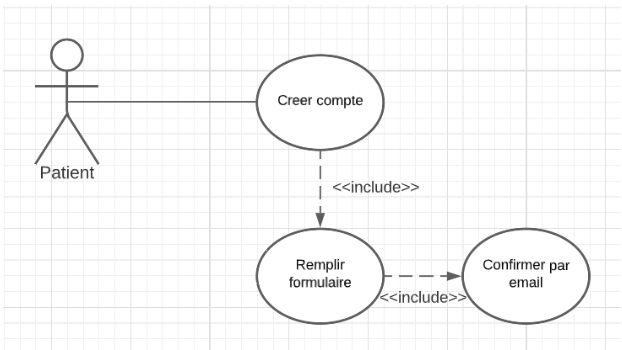
\includegraphics[width=0.5\textwidth]{besoins/creer-compte.png}
    \caption{Diagramme de cas d'utilisation : créer un compte}
    \label{fig:DCU1}
\end{figure}

\subsection{S'authentifier}
\begin{figure}[H]
    \vspace{-10pt}
    \centering
    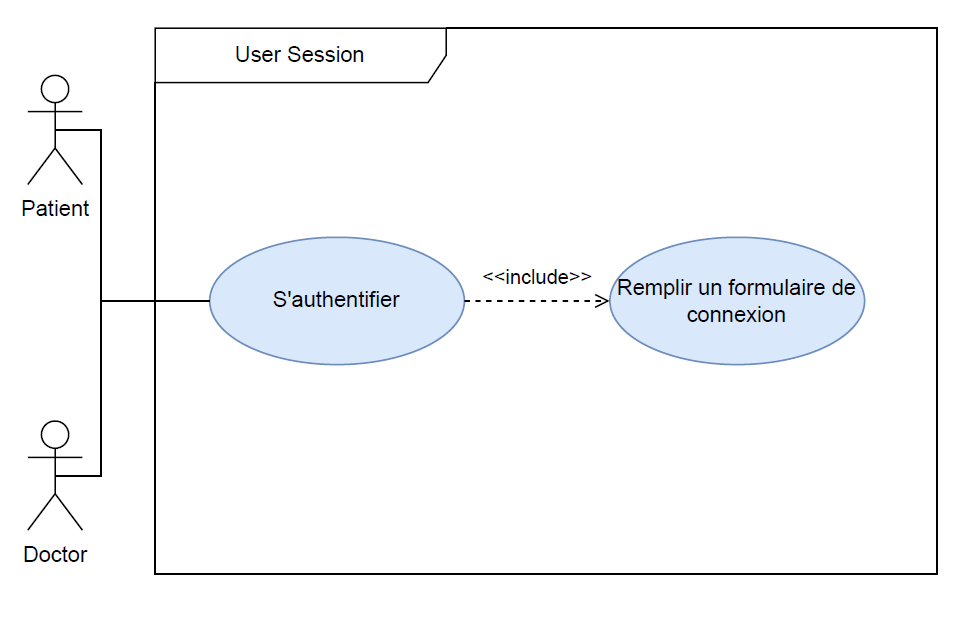
\includegraphics[width=0.5\textwidth]{besoins/authentification.png}
    \caption{Diagramme de cas d'utilisation : s'authentifier}
    \label{fig:DCU2}
\end{figure}

\subsection{Gérer les rendez-vous en ligne (Patient)}
\begin{figure}[H]
    \vspace{-10pt}
    \centering
    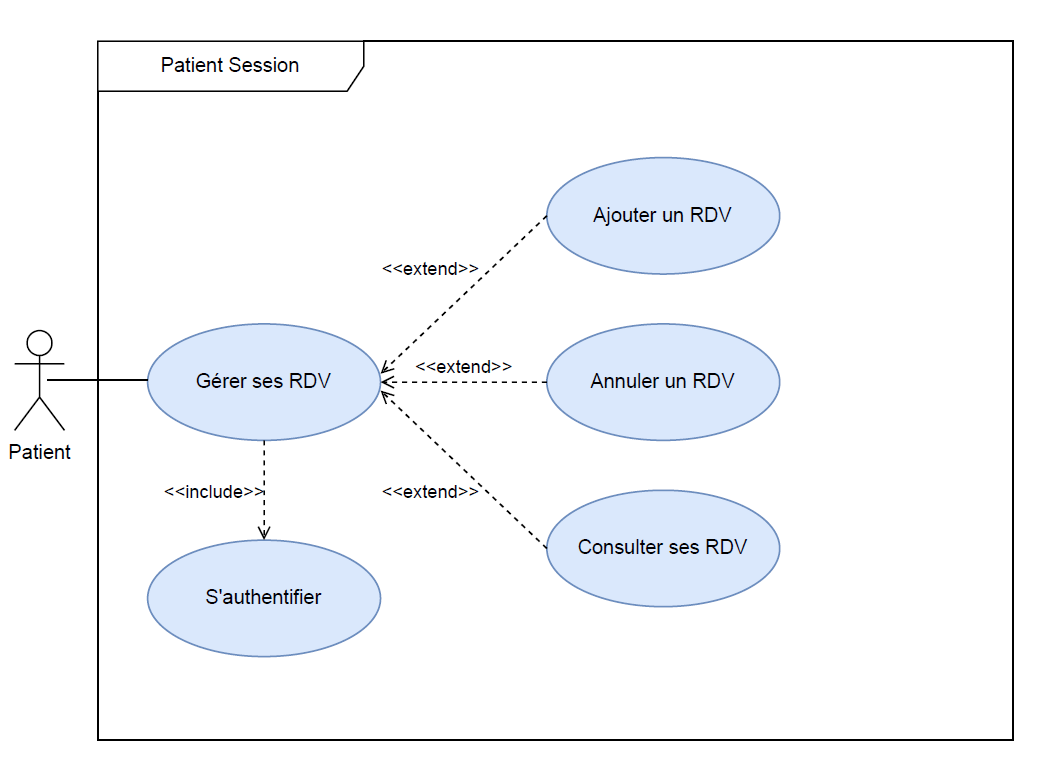
\includegraphics[width=0.5\textwidth]{besoins/gerer-rdv-patient.png}
    \caption{Diagramme de cas d'utilisation : Gérer les rendez-vous en ligne (Patient)}
    \label{fig:DCU3}
\end{figure}

\subsection{Gérer les rendez-vous en ligne (Médecin)}
\begin{figure}[H]
    \vspace{-10pt}
    \centering
    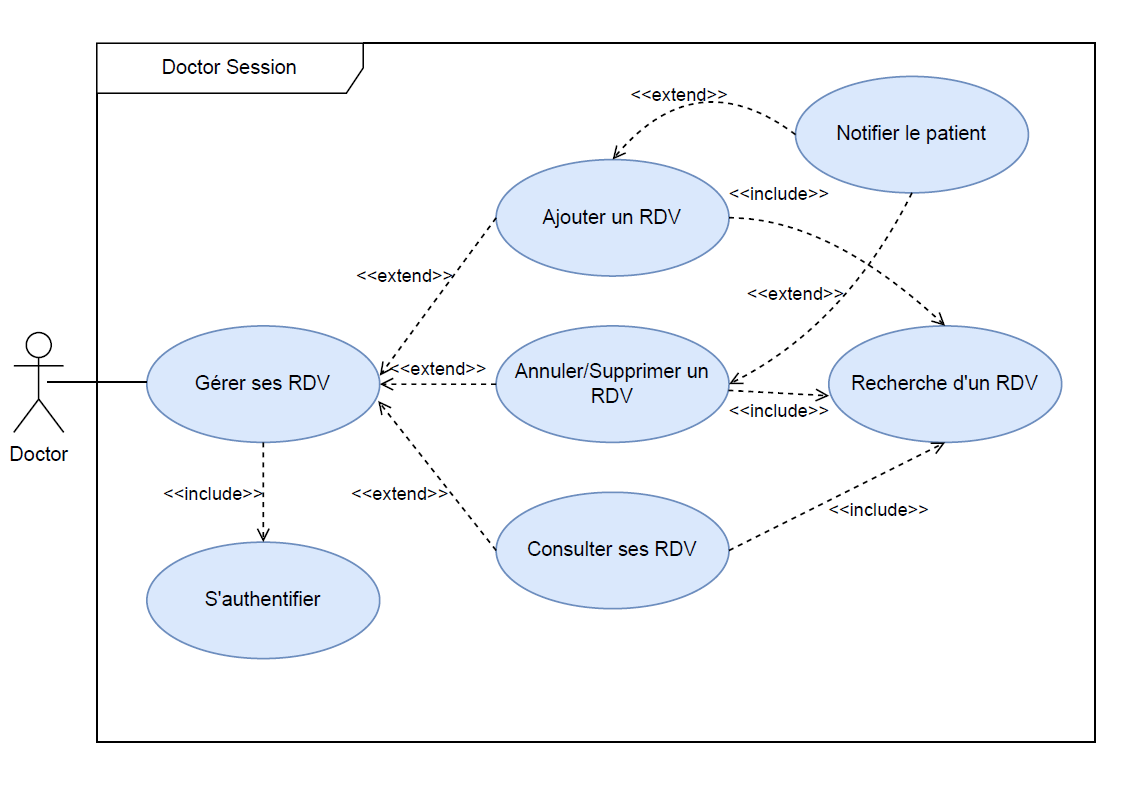
\includegraphics[width=0.5\textwidth]{besoins/gerer-rdv-medecin.png}
    \caption{Diagramme de cas d'utilisation : Gérer les rendez-vous en ligne (Médecin)}
    \label{fig:DCU4}
\end{figure}

\subsection{Consulter les rendez-vous}
\begin{figure}[H]
    \vspace{-10pt}
    \centering
    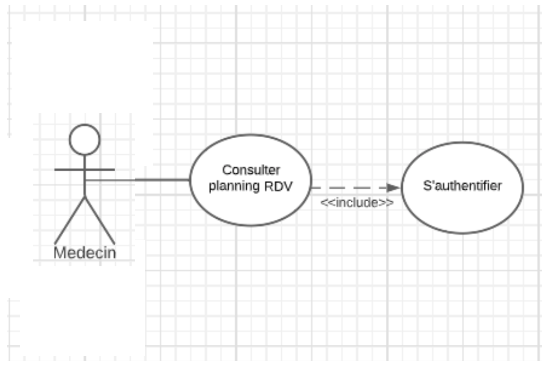
\includegraphics[width=0.55\textwidth]{besoins/consulter-rdv.png}
    \caption{Diagramme de cas d'utilisation : Consulter les rendez-vous}
    \label{fig:DCU5}
\end{figure}

\subsection{Consulter le dossier médical}
\begin{figure}[H]
    \vspace{-10pt}
    \centering
    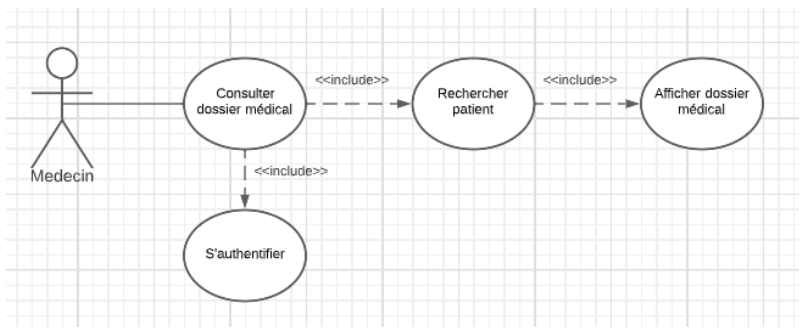
\includegraphics[width=0.6\textwidth]{besoins/consulter-dossier-medical.png}
    \caption{Diagramme de cas d'utilisation : Consulter le dossier médical}
    \label{fig:DCU6}
\end{figure}

\subsection{Gérer le dossier médical}
\begin{figure}[H]
    \vspace{-10pt}
    \centering
    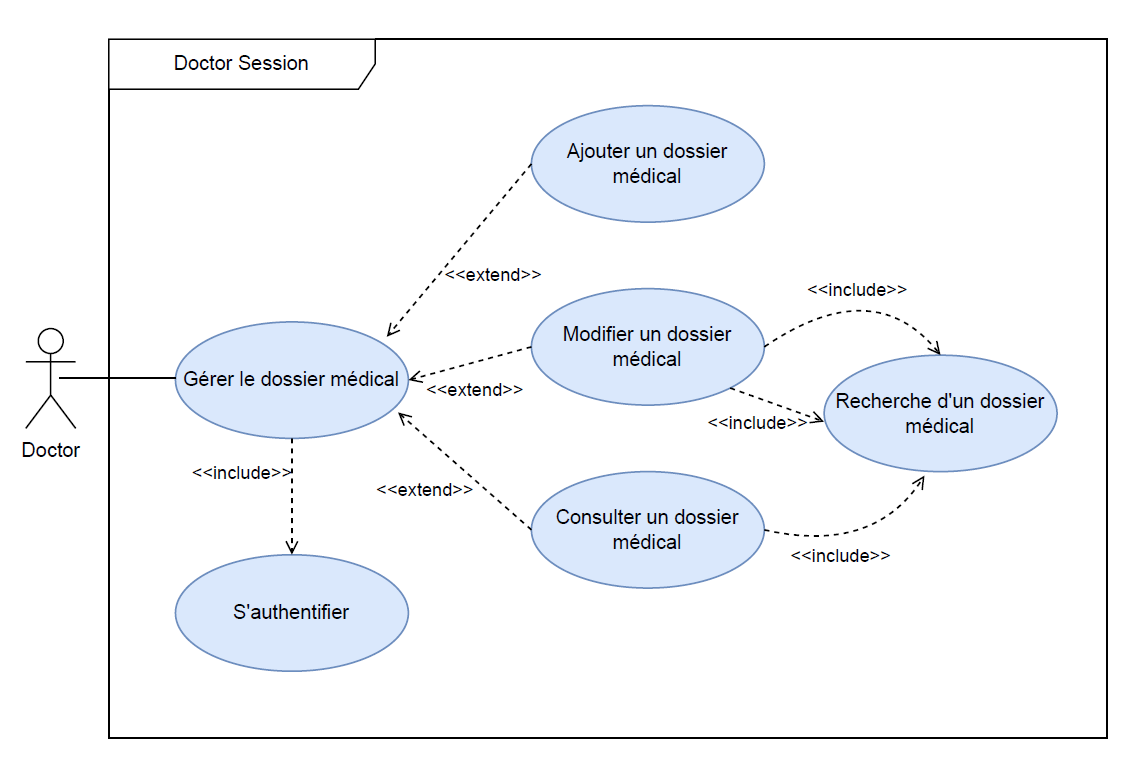
\includegraphics[width=0.5\textwidth]{besoins/gerer-dossier-medical.png}
    \caption{Diagramme de cas d'utilisation : Gérer le dossier médical}
    \label{fig:DCU7}
\end{figure}

\subsection{Génerer le bilan de santé}
\begin{figure}[H]
    \vspace{-10pt}
    \centering
    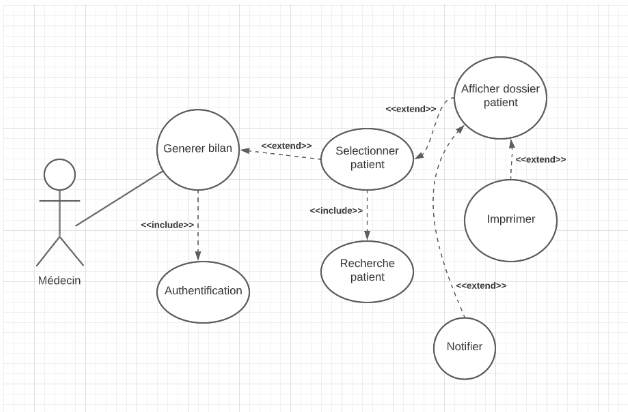
\includegraphics[width=0.5\textwidth]{besoins/bilan-sante.png}
    \caption{Diagramme de cas d'utilisation : Génerer le bilan de santé}
    \label{fig:DCU8}
\end{figure}


\chapter{Conception et Réalisation}


L'architecture logicielle de notre application web pour la gestion d'un cabinet médical se compose d'un front-end, d'un back-end et d'une base de données.
Pour le back-end, nous avons décidé d'utiliser une architecture DDD (Domain-Driven Design) qui se compose de quatre couches distinctes: une couche domaine, 
une couche infrastructure, une couche application et une couche interface utilisateur. \newline \newline
Dans la couche domaine, on trouve les objets metiers qui representent les éléments clés de notre application tels que les patients, les médecins, les rendez-vous, les créneaux horaires, les consultations, 
les adresses des patients et les prescriptions médicales. 
Nous avons distingué les "values object" des Entity et de notre Aggrégat, le dossier médical. Ainsi, nous pouvons recréer nos objets en les récupérant de la base de données ou
alors sauvegarder ces objets. C'est ce qui nous permet de faire le pont entre la base de données et le frontend qui reçoit et met en forme les données.\newline \newline
Nous avons également mis en place une couche infrastructure en utilisant des bases de 
données relationnelles pour stocker les informations de l'application. Cette couche infrastructure est responsable de créer 
pour chaque classe du domaine une table et de gérer les requêtes et les mises à jour dans celles-ci. \newline \newline
Dans la couche interface utilisateur, on a des controllers qui servent d'intérmédiaires entre la partie client et la partie serveur. 
Les controllers reçoivent les entrées utilisateurs, les envoient à la couche application et envoient une réponse au client. Les controllers renvoient en général
une réponse HTTP afin de distinguer les différents code HTTP que l'on reçoit (ok, forbiden...) \newline \newline
Avec cette architecture DDD, nous avons créé une application structurée pour répondre aux besoins spécifiques au cahier des charges. Le code est ainsi plus facile à lire
car les données sont structurées par couches.\newline\newline
Concernant le frontend, nous nous occupons ici de présenter les données, et c'est donc une partie de conception graphique et de présentation aux utilisateurs et non pas une partie
de conception d'un modèle pour la modélisation du cabinet médical. Les données sont donc traitées dans le backend pour pouvoir être stockées dans la base de données.

\section{Diagrammes de classe du Domain}
Concernant le diagramme de classe, nous avons représenté seulement les classes du Domain car elle représente le coeur de l'architecture DDD.
\begin{figure}[H]
    \vspace{-10pt}
    \centering
    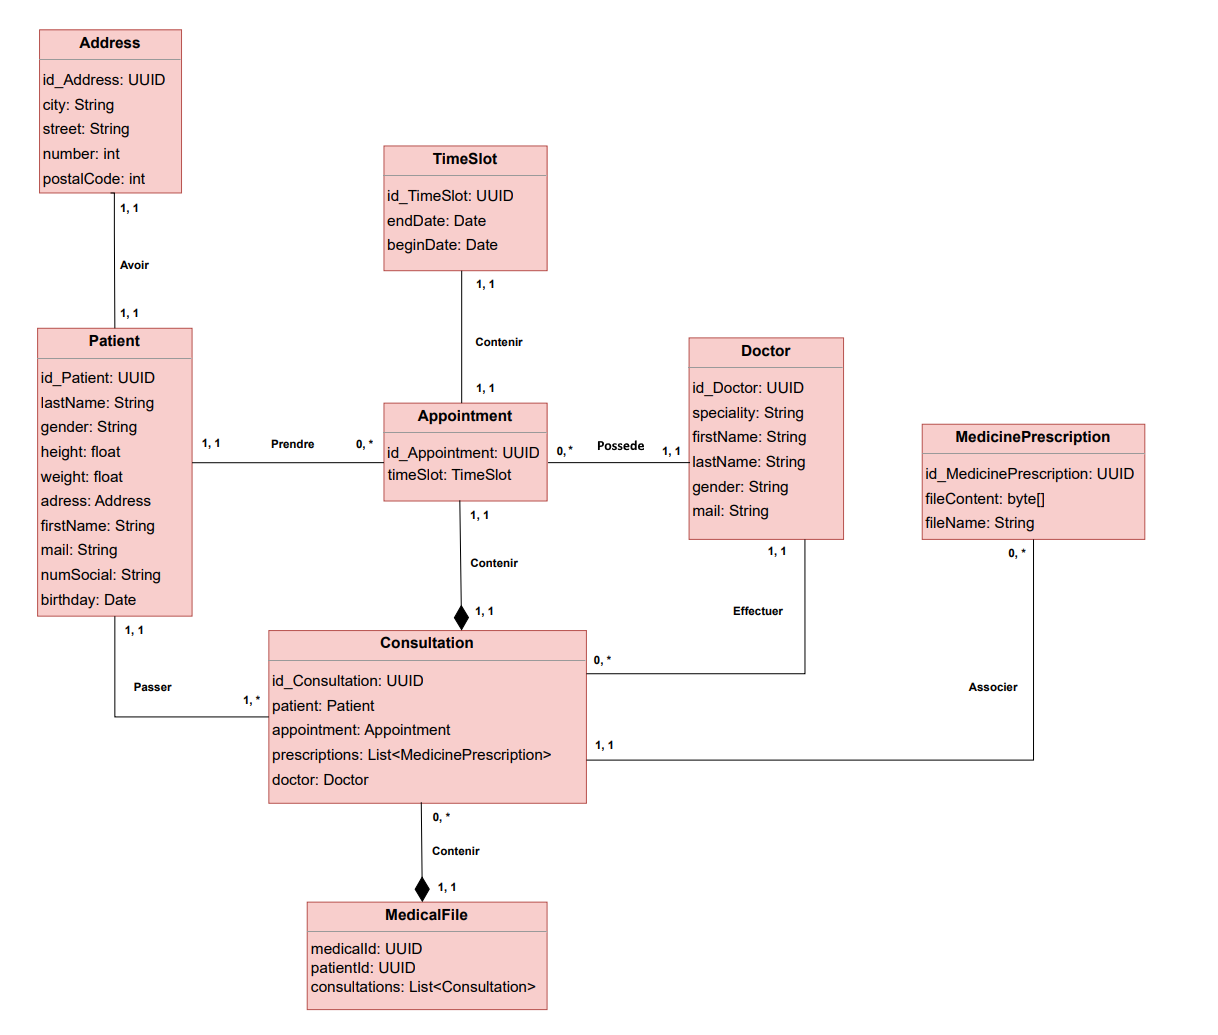
\includegraphics[width=0.85\textwidth]{besoins/class_diagram.png}
    \caption{Diagramme de classes}
    \label{fig:DCU9}
\end{figure}

\section{Passage au modèle relationnel}
Le modèle relationnel est le modèle logique de données qui correspond à l'organisation des données dans les bases de données relationnelles.
Un modèle relationnel est composé de relations, appelée table. Ces tables sont décrites par des attributs ou champs.Pour décrire une relation, on indique tout simplement son
nom, suivi du nom de ses attributs entre parenthèses. L'identifiant d'une relation
est composé d'un ou plusieurs attributs qui forment la clé primaire. Une relation
peut faire référence à une autre en utilisant une clé étrangère, qui correspond à
la clé primaire de la relation référencée. 


\subsection{Passage au modèle relationnel}

A partir du modèle de classes UML de notre application, nous avons obtenu notre modèle
relationnel en appliquant les règles de passage suivantes :

R1 : chaque entité (classe) devient une relation ayant un identiant comme clé primaire.

R2 : une association (X, n). . . (X, 1) (association père fils) provoque la migration d'une
clé primaire, l'identiant coté (X, 1) migre vers l'entité coté (X, n) comme étant une clé
étrangère.

R3 : une association 1..1 dans ce cas on choisit une classe et sa clé migre dans la seconde
comme étant clé étrangère.

R4 : dans le cas de la composition la clé primaire du composé migre vers le composant
et devient à la fois une clé primaire et étrangère.


\subsection{Modèle logique de données}
En appliquant les règles de passages pour notre diagramme de classes, nous
aboutissons au schéma relationnel suivant :
\begin{figure}[H]
    \vspace{-10pt}
    \centering
    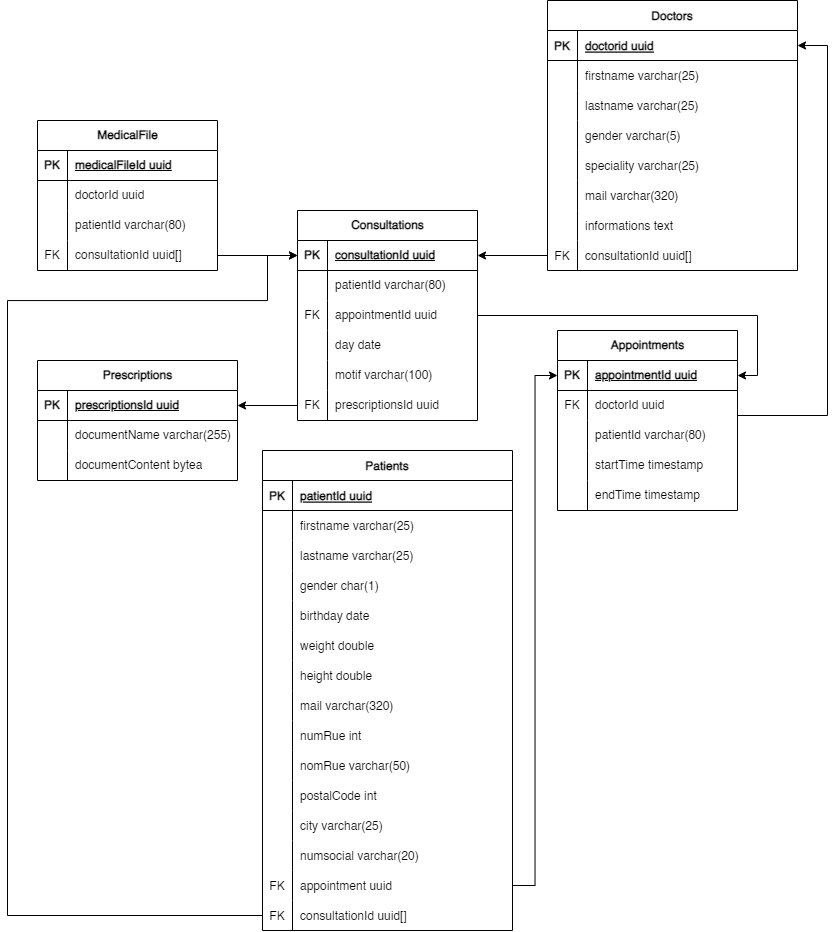
\includegraphics[width=0.85\textwidth]{besoins/modele_relationnel.png}
    \caption{Schéma Relationnel}
    \label{fig:SR}
\end{figure}

\section{Outils de développement}

\begin{itemize}
    \item[$\bullet$] \underline{Java} : Nous avons utilisé le langage de programmation orienté objet Java pour notre projet \cite{JavaSE17API}. \newline
    \item[$\bullet$] \underline{ReactJS} : Pour le côté Front-end, nous avons utilisé la bibliothèque JavaScript ReactJS qui est très populaire dans le monde du développement web et 
    très facile d'utilisation. Elle fonctionne avec des composants où chaque composant représente une partie de l'interface utilisateur. Ces composants sont réutilisables ce qui nous permet de gagner du temps. 
    Elle possède également une documentation bien organisée et facile à comprendre \cite{ReactJS}. \newline
    \item[$\bullet$] \underline{Maven} : Pour la construction du projet nous avons choisi Maven, un outil de gestion de projet facile à configurer et à utiliser. Il peut être étendu grâce à des plugins pour répondre à des besoins spécifiques. \cite{ApacheMaven}\newline
    \item[$\bullet$] \underline{Springboot} : Pour créer notre application web, nous avons décidé d'utiliser Spring Boot qui est un framework Java qui fournit un ensemble de fonctionnalités prêtes à l'emploi pour simplifier la configuration, 
    le déploiement et la gestion des applications web \cite{springboot}. \newline 
    \item[$\bullet$] \underline{Git} : Pour pouvoir au mieux travailler sur ce projet chacun de notre côté, nous avons décidé d'utiliser Git qui est un logiciel de gestion de versions décentralisé. Il permet de travailler
    sur des parties différentes du code en même temps et il est très utile pour le travail en équipe \cite{GitDocumentation}.\newline
    \item[$\bullet$] \underline{Postgresql} : Pour la gestion de notre base de données nous avons utilisé Postgresql qui est un système de gestion de bases de données relationnelles. Il est fiable et robuste, de plus 
    nous avions déjà utilisé ce système donc c'était facile pour nous de l'utiliser pour notre projet \cite{postgresql_doc}. \newline
    \item[$\bullet$] \underline{JUnit} : Pour les tests, nous avons utilisé JUnit qui est un framework de test unitaire pour Java et qui permet de tester des fragments de code de manière isolée et automatisée \cite{JUnit5}.\newline
\end{itemize}

\section{Côté back-end}

Pour la partie back-end, nous avons entamé le processus par l'implémentation de la couche domaine en y incluant les protagonistes majeurs 
du cabinet médical : les docteurs et les patients. Nous avons poursuivi notre travail en créant des value objects et des 
entités tels que les adresses postales, les rendez-vous, les consultations, les ordonnances et les utilisateurs. Nous avons conclu en créant l'agrégat, qui est un dossier médical. \newline\newline
Ensuite, nous avons développé la couche infrastructure en créant quatre dépôts distincts : un pour les médecins, un pour les 
patients, un pour les utilisateurs et un pour le cabinet médical dans son ensemble. Ces dépôts contiennent les requêtes et les 
insertions dans les tables de la base de données.\newline\newline
Par la suite, nous avons travaillé sur la couche application, qui récupère les informations de la couche infrastructure afin de les transmettre à la couche interface utilisateur. \newline\newline
Enfin, nous avons implémenté la couche interface utilisateur, dans laquelle se trouvent des contrôleurs pour les patients, les médecins et les utilisateurs qui font le lien entre la partie 
serveur et la partie client.\newline

\section{Côté front-end}

Le développement de l'interface utilisateur de notre application web a été effectué en utilisant React JS. Ce framework a permis de créer une 
interface utilisateur attrayante et réactive pour les utilisateurs. \newline\newline
Nous avons commencé par concevoir la page principale, qui comprend une liste 
déroulante permettant aux utilisateurs de sélectionner la spécialité du médecin recherché (Dentiste, Généraliste, etc.). \newline\newline
Ensuite, nous avons créé les pages d'inscription et de connexion pour permettre aux patients de se connecter à leur compte ou d'en créer un nouveau.
Une partie d'administration a également été développée, avec un router dédié permettant d'accéder à toutes les pages disponibles pour les patients 
connectés, telles que la page "Mes rendez-vous", "Mes documents" et "Mon compte", où les patients peuvent modifier leurs informations personnelles. 
Un header a également été ajouté pour faciliter la navigation entre ces différentes pages.\newline\newline
Dans la partie publique de l'application, accessible à tous les utilisateurs, y compris ceux qui ne sont pas connectés, nous avons créé des pages 
dédiées à chaque médecin pour afficher les créneaux horaires disponibles. Nous avons ensuite créé une partie réservée uniquement aux médecins, où 
ils peuvent accéder à leur planning, visualiser leurs patients et modifier leurs informations personnelles. \newline
Pour appliquer ceci, nous avons définit un router grâce au module React.Router permettant de gérer les routes de notre application web en fonction des URL qui sont appelées par l'utilisateur. En d'autres termes, le router permet de faire correspondre une URL donnée à un composant spécifique dans l'application.
Cette méthode nous permet également de gérer les redirections et les transitions d'une page à l'autre, pour gérer l'historique de navigation et les paramètres d'URL, et pour autoriser ou refuser l'accès à certaines pages en fonction des autorisations de l'utilisateur.

\section{Base de données}

Nous avons créé une base de données à l'aide du système Postgresql dans laquelle nous avons ajouté des tables pour chaque classe de notre domaine DDD.\newline
\begin{itemize}
    \item \textbf{Table doctors} : on stocke les informations relatives aux docteurs comme leur nom, prénom, spécialité et les informations qu'on retrouve sur leur page Medicolib.\newline
    \item \textbf{Table patients} : on stocke les informations personnelles des patients comme leur nom, prénom, genre, poids, taille, adresse mail et date de naissance. \newline
    \item \textbf{Table address} : on stocke les différentes parties d'une adresse postale d'un patient tel que le numéro et nom de la rue, le code postal et le nom de la ville. \newline
    \item \textbf{Table users} : on stocke les adresses mails et mots de passe cryptés des utilisateurs ainsi que leur rôle (patient ou doctor). \newline
    \item \textbf{Table availableTimeSlots} : on stocke les créneaux de rendez-vous disponibles pour chaque médecin. \newline
    \item \textbf{Table appointments} : on stocke tous les rendez-vous pris pour chaque médecin et chaque patient. \newline
    \item \textbf{Table documents} : on stocke les documents que les patients peuvent ajouter en amont de leur rendez-vous. \newline
    \item \textbf{Table consultations} : on stocke les informations d'une consultation entre un médecin et un patient et un identifiant d'ordonnance si il y en a une à la suite de la consultation. \newline
    \item \textbf{Table prescriptions} : on stocke les ordonnances que le médecin prescrit au patient. \newline
    \item \textbf{Table medicalFile} :  on stocke les dossiers médicaux des patients pour chaque médecin, qui correspondent à une liste de leurs consultations. \newline
    \item \textbf{Table price} : on stocke le prix des services proposés pour tous les médecins c'est-à-dire l'identifiant du docteur avec l'intitulé de la prestation et le prix. \newline
\end{itemize}

\chapter{Tests}


Nous allons maintenant aborder la partie sur les tests. Nous avons utiliser JUnit pour effectuer des tests unitaires sur les contrôleurs. JUnit est un framework permettant de développer des tests unitaires
automatisables. Ainsi, nous pouvous nous assurer que le code répond toujours aux besoins après avoir implémenté ou effectué des modifications. Ces tests correspondent à des assertions qui permettent de tester les résultats 
attendus. L'objectif ici, est de tester les méthodes des différents contrôleurs que nous avons implémentés pour vérifier que le code que nous avons produit est bien correct.
Les tests sont séparés du code de la classe permettant ainsi de la tester. Le principe d'implémentation de ces tests est le suivant : \newline
\begin{itemize}
    \item[$\bullet$] Création d'une instance du contrôleur et de tout autre objet nécessaire aux tests
    \item[$\bullet$] Appel de la méthode à tester
    \item[$\bullet$] Comparaison du résultat attendu avec le résultat que l'on vient d'obtenir \newline
\end{itemize}
L'avantage est de pouvoir écrire un certain nombre de tests permettant de tester chacun différents cas de figure et de trouver le plus de bugs possibles dans notre application.
Nous utilisons également, des objets Mock (du framework Mockito). MockMvc est en fait un objet de Spring \cite{spring_testing_web} permettant de simuler un objet qu'on aura besoin d'utiliser pour effectuer nos tests. Cela permet notamment, de simuler
des accès à la base de données.
Tout cela nous permet ainsi de rédiger nos tests sur les contrôleurs. Nous pouvons ainsi vérifier que les reqûetes effectuées et les objets retournés et/ou intégrés dans la base de données
sont conformes au résultat attendu.
Nous avons trois contrôleurs donc trois classes de tests correspondantes.

\subsection{UserControllerTest}
Cette section correspond aux tests sur toute la partie "connexion" de notre site web. Plus précisement, nous testons ici que les connexions et rénitialisation de mot de passe s'effectuent bien.
Nous avons effectué des tests positifs et négatifs, c'est-à-dire avec des bons identifiants de connexion et des mauvais et nous nous s'assurons que les réponses HTTP renvoyées sont bien identiques.
Par exemple, si un utilisateur se connecte avec un mauvais mot de passe, il faut que la réponse attendue soit "Forbiden". Ainsi, si un des tests ne passent pas, il est simple de savoir où l'erreur se produit.
Voici un exemple d'un de nos tests pour vérifier qu'un utilisateur ne peut pas rénitialiser son mot de passe s'il n'est pas enregistré en tant qu'utilisateur (qu'il n'a pas de compte).
\begin{lstlisting}
    @Test
    public void testResetPasswordWithNonUser() throws Exception {
        Map<String, String> map = new HashMap<>();
        map.put("mail", "test@gmail.com");

        when(medicalPractice.checkUserExist("test@gmail.com")).thenReturn(false);

        mockMvc.perform(post("/new-password")
                .contentType(MediaType.APPLICATION_JSON)
                .content(asJsonString(map)))
                .andExpect(status().isNotFound());
    }
\end{lstlisting}



\subsection{PatientControllerTest}
Cette section va correspondre aux tests du controleur du patient et va comme précédemment, tester les différentes fonctionnalités de l'API Rest (avec les codes HTTP).
Nous testons ainsi toutes les demandes liées aux patients : modifications d'informations, prises et annulations de RDV, ajout de documents, etc. Comme précédemment, nous avons, pour certaines méthodes,
tester plusieurs cas, lorsque la méthode en question peut retourner une réponse "ok" ou "forbiden".
Voici un exemple d'un de nos tests pour vérifier qu'un utilisateur peut supprimer un document : 
\begin{lstlisting}
    @Test
    void testDeleteDocument() throws SQLException, IOException {
        HashMap<String, String> mockMap = new HashMap<>();
        mockMap.put("apptid", "94b9b73a-f561-4ca9-a6c3-6ae7e0361773");
        mockMap.put("mail", "johndoe@gmail.com");
        MockMultipartFile file = new MockMultipartFile("test", "test.txt", "text/plain", "file content".getBytes());
        patientController.uploadFile(file, mockMap.get("mail"), mockMap.get("apptid"));
        HashMap<String, String> map = new HashMap<>();
        map.put("id", "94b9b73a-f561-4ca9-a6c3-6ae7e0361773");
        map.put("name", file.getName());
        ResponseEntity<String> response = patientController.deleteDocument(map);
        assertEquals(HttpStatus.OK, response.getStatusCode());
        assertEquals("File deleted successfully", response.getBody());
    }
\end{lstlisting}

\subsection{DoctorControllerTest}
Cette section va correspondre aux tests du controleur concernant les docteurs. Nous allons, comme précédemment effectuer des tests sur les différentes méthodes du contrôleur et plus précisement sur les points suivants :
la consultation du planning par le docteur, l'ajout de consultations, l'annulation de RDV etc.
Voici un exemple de test pour récupérer la liste des patients d'un docteur : \newline
\begin{lstlisting}
    @Test
    void testGetAllPatientByDoctor() throws ParseException, SQLException {
        SimpleDateFormat format = new SimpleDateFormat("yyyy-MM-dd");
        Date date = format.parse("2023-04-03");
        List<Patient> expectedPatients = new ArrayList<>();
        Patient patient = new Patient(
            UUID.fromString("dccf9cfd-f2cc-4e44-8357-dd4140e17b73"),
            "John" , "Doe", "M", date, "54165", "johndoe@gmail.com", null, 0, 0);
        expectedPatients.add(patient);
        Map<String, String> requestBody = new HashMap<>();
        requestBody.put("mail", "doctor@gmail.com");
        when(medicalPractice.getPatientsByDoctor(medicalPractice.getInformationsDoctorByMail("doctor@gmail.com"))).thenReturn(expectedPatients);
        ResponseEntity<List<Patient>> response = doctorController.getAllPatientByDoctor(requestBody);
        assertEquals(HttpStatus.OK, response.getStatusCode());
        assertEquals(expectedPatients, response.getBody()); 
    }
\end{lstlisting}

Pour conclure cette partie sur les tests, nous pouvons dire que les tests représentent une partie très importante du projet car elles nous permettent de suivre l'évolution de notre application
et de détecter des bugs rapidement et lors de l'ajout de nouvelles fonctionnalités. L'avantage de JUnit est que c'est très simple à utiliser, et très rapide à mettre en place et cela nous permet
d'écrire beaucoup de tests permettant de couvrir une grande partie de notre programme.


\chapter{Résultats}

La partie résultats de ce rapport présente les conclusions de notre projet. Dans cette section, nous présentons les fonctionnalités de l'application (les besoins fonctionnels et non fonctionnels), son interface utilisateur, sa sécurité et sa facilité d'utilisation. Nous avons fait au mieux pour établir une mise en relation simple et efficace entre patient et professionnel de santé. Notamment grâce à une prise de rendez-vous simple et intuitive selon les besoins des patients mais aussi permettre aux professionnels de santé de pouvoir suivre les dossiers médicaux de chacun de leurs patients et avoir une vue générale sur l'ensemble de leurs rendez-vous sur un planning. Les informations présentées dans cette section ont été obtenues à partir d'une étude approfondie des besoins, d'une analyse comparative d'autres applications similaires et d'une phase de conception et de développement rigoureuses. Nous sommes convaincus que cette application représente une solution efficace et facile d'utilisation pour la gestion des cabinets médicaux et qu'elle répondra aux besoins spécifiques des professionnels de santé et de leurs patients. En effet, nous avons conceptualisé au mieux cette application en proposant un \textit{responsive web design}, permettant à l'application de s'adapter à toutes les tailles de fenêtres.
\newline
\newline

\section{\noindent Navigation en tant que \textit{Visiteur} {\fontsize{12}{16}\selectfont(Utilisateur non-connecté)}: }

\subsection{Fonctionnalité de l'entête (Header):}
    \begin{itemize} 
        \item[$\bullet$] Cliquer sur se connecter pour être redirigé vers la page \textit{\hyperref[login]{Login}}.
    \end{itemize}
    \vspace{3mm}

\subsection{Fonctionnalité de la page d'Accueil (Homepage):}\label{homepage}
    \begin{itemize}
        \item[$\bullet$] Se renseigner sur la nature du site, les services qu’il propose et la qualité de ces services.
        \item[$\bullet$] Utiliser la barre de navigation :
        \begin{itemize}
            \item Rechercher sans spécifier une spécialité médicale : redirection vers la page \textit{\hyperref[docteurs]{Docteurs}} en  répertoriant l’ensemble des praticiens du cabinet, toute spécialité confondue.
            \item Rechercher avec une spécialité choisie dans la liste déroulante (qui est à jour en direct, en affichant chaque spécialité disponible selon les médecins enregistrés dans la base de données), et ce par une redirection vers la page \textit{\hyperref[docteurs]{Docteurs}} répertoriant les praticiens correspondant à la spécialité recherchée.
        \end{itemize}
    \end{itemize}
    \vspace{3mm}

\subsection{Fonctionnalité de la page repertoriant les docteurs (Docteurs):}\label{docteurs}
    \begin{itemize}
        \item[$\bullet$] Cliquer sur le bouton prendre RDV pour accéder à la page \textit{\hyperref[docteur]{Docteur}} (page personnelle du docteur).
        \item[$\bullet$] Naviguer sur le planning, en changeant de semaine pour trouver un jour et un créneau.
        \item[$\bullet$] Afficher toutes les horaires des jours de la semaine choisie.
        \item[$\bullet$] Prendre directement un rendez-vous sur le planning selon disponibilité (les créneaux déjà reservés ne sont pas affichés), en cliquant sur un créneau, l’utilisateur sera alors redirigé vers la page \textit{\hyperref[login]{Login}} car il est impossible de réserver un créneau si l'utilisateur n'est pas connecté.
    \end{itemize}
    \vspace{3mm}

\subsection{Fonctionnalité de la page personnel d'un médecin (Docteur):}\label{docteur}
    \begin{itemize}
        \item[$\bullet$] Consulter les informations pratiques du docteur en question (tarifs, informations, contact).
        \item[$\bullet$] Naviguer sur le planning pour trouver un jour et un créneau.
        \item[$\bullet$] Prendre un rendez-vous sur le planning selon disponibilité (les créneaux déjà reservés seront affichés mais barrés et non cliquable), en cliquant sur un créneau, l’utilisateur sera alors redirigé vers la page \textit{\hyperref[login]{Login}}.
    \end{itemize}
    \vspace{3mm}

\subsection{Fonctionnalité de la page de connexion (Login):}\label{login}
    \begin{itemize}
        \item[$\bullet$] Se connecter via son email et son mot de passe (que l’on peut masquer ou non). {\fontsize{8}{14}\selectfont Remarque: le mot de passe est stocké de manière crypté dans la base de données grâce à un encodage de celui-ci, definit par sa valeur de hashage.}
        \item[$\bullet$] Indiquer "mot de passe oublié", ce qui nous invite à entrer notre email pour recevoir un mail contenant un nouveau mot de passe aléatoire. {\fontsize{8}{14}\selectfont Remarque: si le mail n'existe pas dans la base de données, alors aucun mail ne sera envoyé.}
        \item[$\bullet$] Cliquer sur "Enregistrez-vous", ce qui redirigera l'utilisateur sur la page \textit{\hyperref[register]{Register}}.
    \end{itemize}
    \vspace{3mm}

\subsection{Fonctionnalité de la page de création de compte (Register):}\label{register}
    \begin{itemize}
        \item[$\bullet$] Renseigner l'intégralité des informations demandées pour créer son compte en tant que patient (les professionnels sont ajoutés par le biais des administrateurs), puis se connecter.
    \end{itemize}

\vspace{1.5cm}


\section{\noindent Navigation en tant que \textit{Patient} {\fontsize{12}{16}\selectfont(connecté)}: }
\vspace{0.6cm}

\subsection{Fonctionnalité de l'entête (Header):}\label{header}
    \begin{itemize}
        \item[$\bullet$] Cliquer sur "Mes rendez-vous" pour être redirigé vers la page \textit{\hyperref[appointments]{Appointments}}.
        \item[$\bullet$] Cliquer sur "Mes documents" pour être redirigé vers la page \textit{\hyperref[documents]{Documents}}.
        \item[$\bullet$] Cliquer sur le prénom pour faire apparaitre une liste déroulante:
        \begin{itemize}
            \item Cliquer sur "Mon compte" pour être redirigé vers la page \textit{\hyperref[edit]{Edit}}.
            \item Cliquer sur "Déconnexion" pour être déconnecté et fermer la session.
        \end{itemize}
        \item[$\bullet$] Si la taille de la page est réduite, tous les boutons du header se retrouve dans la liste déroulante en cliquant sur son prénom.
    \end{itemize}
    \vspace{3mm}

\subsection{Fonctionnalité de la page d'Accueil (Homepage):}
    \begin{itemize}
        \item[$\bullet$] Décrite dans la partie \textit{\hyperref[homepage]{6.1.2}}.
    \end{itemize}
    \vspace{3mm}

\subsection{Fonctionnalité de la page repertoriant les docteurs (Docteurs):}\label{docteurs2}
    \begin{itemize}
        \item[$\bullet$] Décrite dans la partie \textit{\hyperref[docteurs]{6.1.3}}.
        \item[$\bullet$] Cependant il est désormais possible de réserver un créneau car le patient est connecté, il sera alors redirigé vers la page \textit{\hyperref[appointments]{Appointments}}. {\fontsize{8}{14}\selectfont Remarque: le patient recevra un mail lui indiquant que son rendez-vous à la date X et l’horaire Y a été réservé}.
    \end{itemize}
    \vspace{3mm}

\subsection{Fonctionnalité de la page personnel d'un médecin (Docteur):}\label{docteur2}
    \begin{itemize}
        \item[$\bullet$] Décrite dans la partie \textit{\hyperref[docteur]{6.1.4}}.
        \item[$\bullet$] Cependant il est désormais possible de réserver un créneau car le patient est connecté, il sera alors redirigé vers la page \textit{\hyperref[appointments]{Appointments}}. {\fontsize{8}{14}\selectfont Remarque: le patient recevra un mail lui indiquant que le rendez-vous à la date X et l’horaire Y a été réservé}.
    \end{itemize}
    \vspace{3mm}

\subsection{Fonctionnalité de la page des rendez-vous (Appointments):}\label{appointments}
    \begin{itemize}
        \item[$\bullet$] Affiche les rendez vous à venir pris par le patient, si aucun rendez vous n’est planifié alors un message sera affiché pour indiquer au patient qu’aucun rendez vous n’est planifié pour le moment.
        \item[$\bullet$] Possibilité de cliquer sur “voir mes rendez-vous passés” pour afficher les rendez-vous passés, si aucun rendez-vous n’est passé, de même un message sera présent pour prévenir le patient. {\fontsize{8}{14}\selectfont Remarque: au bout d’un an les rendez vous passés ainsi que les documents qu’ils comportent seront effacé}.
        \item[$\bullet$] Ajouter des documents pour un rendez-vous, ils seront alors répertoriés sur la page \textit{\hyperref[documents]{Documents}}. {\fontsize{8}{14}\selectfont Remarque: les documents ajoutés seront visibles uniquement par le médecin indiqué sur le rendez-vous}.
        \item[$\bullet$] Annuler un rendez vous, par conséquent le créneau disparaitra de la page, le rendant à nouveau disponible pour d’autres patients. {\fontsize{8}{14}\selectfont Remarque: un mail sera alors envoyé indiquant que le rendez vous à la date X et l’horaire Y a été annulé}.
    \end{itemize}
    \vspace{3mm}

\subsection{Fonctionnalité de la page des documents (Documents):}\label{documents}
    \begin{itemize}
        \item[$\bullet$] Affiche tous les documents déposés par le patient avec la date de la consultation concernée, avec possibilité de télécharger le document ou de le retirer (ce qui va le retirer pour le praticien également).
        \item[$\bullet$] Affiche les ordonnances prescrite par le praticien avec la date de la consultation concernée, il est possible de la télécharger sous le format pdf.
        \item[$\bullet$] Si aucun document n’est disponible alors un message sera affiché pour indiquer au patient qu’aucun document n’est disponible pour le moment.
    \end{itemize}
    \vspace{3mm}

\subsection{Fonctionnalité de la page du compte (Edit):}\label{edit}
    \begin{itemize}
        \item[$\bullet$] Modifier les informations personnelles: prénom, nom, numéro de sécurité sociale et adresse postale. {\fontsize{8}{14}\selectfont Remarque: le prénom et nom sera parsé sous la forme Xxxxx et Xxxxx permettant une bonne lisibilité des informations. De plus, si le patient souhaite modifier son adresse et que celle-ci n'est pas complète, elle ne sera pas prise en compte, en laissant l’ancienne adresse.}
        \item[$\bullet$] Modifier les informations médicale: sexe, date de naissance, poids et taille. {\fontsize{8}{14}\selectfont Remarque: il n’est pas possible de rentrer une date de naissance supérieure à la date actuelle}.
        \item[$\bullet$] Modifier les informations de connexion: mail et mot de passe.
        \item[$\bullet$] Enregistrer les modifications, une notification apparaîtra alors sur l'écran à la suite de la requête axios pour indiquer la bonne prise en compte des modifications.
        \item[$\bullet$] Supprimer le compte, un pop-up apparaîtra demandant une confirmation, à la suite de cette confirmation le patient sera déconnecté et le compte supprimé.
    \end{itemize}

\vspace{1.5cm}

\section{{\noindent Navigation en tant que \textit{Docteur} {\fontsize{12}{16}\selectfont(connecté)}: }}
\vspace{0.6cm}

\subsection{Fonctionnalité de l'entête (Header):}\label{header2}
    \begin{itemize}
        \item[$\bullet$] Cliquer sur "Planning" pour être redirigé vers la page \textit{\hyperref[planning]{Planning}}.
        \item[$\bullet$] Cliquer sur "Mes patients" pour être redirigé vers la page \textit{\hyperref[patients]{Patients}}.
        \item[$\bullet$] Cliquer sur le prénom pour faire apparaitre une liste déroulante:
            \begin{itemize}
                \item Cliquer sur "Mon compte" pour être redirigé vers la page \textit{\hyperref[edit2]{Edit}}.
                \item Cliquer sur "Déconnexion" pour être déconnecté et fermer la session.
            \end{itemize}
        \item[$\bullet$] Si la taille de la page est réduite, tous les boutons du header se retrouve dans la liste déroulante en cliquant sur son prénom.
    \end{itemize}
    \vspace{3mm}
    
\subsection{{Fonctionnalité de la page répertoriant les RDV (Planning)}:}\label{planning}
    \begin{itemize}
        \item[$\bullet$] Se déplacer de semaine en semaine et visualiser tous les jours de la semaine selectionnée.
        \item[$\bullet$] Pouvoir revenir au jour actuel en cliquant sur un bouton "Aujourd'hui" pour faciliter la navigation.
        \item[$\bullet$] Cliquer sur un RDV apparaissant sur le planning (dont on peut prévisualiser le nom, prénom du patient et l'heure du RDV) 
        et ouverture d'un popup avec différentes fonctionnalités :
        \begin{itemize}
            \item Affichage des informations (Nom et prénom du patient, heure et date).
            \item Voir les documents ajoutés par le patient (s'il en a ajouté sinon un message indiquant qu'il n'y a pas de documents apparait) et pouvoir les télécharger.
            \item Cliquer sur un bouton amenant directement au dossier médical du patient.
            \item Cliquer sur un bouton permettant d'ajouter une consultation au patient au moment du RDV.
            \item Pour les RDV qui ne sont pas encore passés, un bouton "Annuler" est disponible permettant ainsi au docteur de pouvoir annuler ce RDV. Une notification est envoyé au patient par mail.
            \item Pouvoir cliquer sur le bouton pour fermer ce popup.\newline
        \end{itemize}
    \end{itemize}
    Le docteur peut voir ses RDV qui sont passés et ceux à venir dans le planning en se déplacant de semaine en semaine. Ainsi, il peut retrouver des documents transmis par le patient même lorsqu'un RDV est passé.
    \vspace{3mm}
    
\subsection{{Fonctionnalité de la page répertoriant les patients d'un docteur (Patients)}:}\label{patients}
Pour qu'un docteur puisse avoir des patients, il faut que ceux-ci prennent un RDV pour la première fois avec ce docteur. Un dossier médical entre le patient et le docteur
est alors créé même si le patient ne reprend plus de RDV après.
\begin{itemize}
    \item[$\bullet$] Si le docteur n'a jamais eu de patients, la page sera vide. Si des patients ont déjà pris RDV avec lui, un tableau de patients est disponible :
    \begin{itemize}
        \item Affichage du nom, prénom, date de naissance, sexe et mail de chaque patient.
        \item Possibilité d'accéder au \textit{\hyperref[dossier médical]{dossier médical}} d'un patient.
    \end{itemize}
    \item[$\bullet$] Les patients sont affichés 10 par 10, donc on peut accéder aux pages suivantes si besoin.
\end{itemize}
\vspace{3mm}
    
\subsection{{Fonctionnalité de la page de consultation du dossier médical d'un patient}:}\label{dossier médical}
\begin{itemize}
    \item[$\bullet$] En haut à gauche : affichage du numéro du dossier médical.
    \item[$\bullet$] Sur la partie gauche de la page, affichage des informations personnelles du patient : Nom, prénom, sexe, date de naissance, taille, poids,
    numéro de sécurité sociale, son adresse et son mail. Pour les informations qui n'ont pas été transmises (le poid par exemple), "non renseigné" apparait.
    \item[$\bullet$] Sur la partie droite de la page, affichage des consultations de ce patient : 
    \begin{itemize}
        \item Si le premier RDV du patient n'est pas encore passé, alors cette partie sera vide car aucune consultation n'aura encore été créée par le médecin.
        \item Si le patient a déjà eu au moins un RDV, alors le docteur a normalement créé une consultation lors de ce RDV. On retrouve ainsi la date de chaque consultation,
        le motif de la venue du patient et les différentes ordonnances si le médecin en a généré (voir en détail \textit{{\hyperref[consultation]{Consultations}}} ). Si des ordonnances
        sont donc présentes, le docteur peut les télécharger. Notons que le docteur ne peut consulter que les consultations qui lui sont liées et non pas les consultations des 
        autres docteurs avec le même patient.
    \end{itemize}
\end{itemize}
\vspace{3mm}
    
\subsection{{Fonctionnalité de la page d'ajout d'une consultation}:}\label{consultation}
\begin{itemize}
    \item[$\bullet$] Lors du RDV, le docteur ajoute une consultation au patient :
    \begin{itemize}
        \item Il peut ajouter la date de la consultation. Par défaut, c'est la date actuelle qui est mise.
        \item Il peut ajouter le motif de la consultation.
        \item Il peut ensuite ajouter une ordonnance ou non. S'il n'ajoute pas d'ordonnance, dans le cas où le patient n'a aucun traitement à prendre et qu'il enregsitre la consultation,
        celle-ci s'ajoute dans la section du {\hyperref[dossier médical]{dossier médical}} du patient. S'il ajoute une ordonnance, des cases de texte apparaissent pour ajouter les différentes
        prescriptions (de médicaments par exemple). On peut ajouter autant de prescriptions que l'on veut. Lorsqu'on enregistre, la consultation est créée avec l'ordonnance qui est générée sous forme d'un fichier pdf.
        Ce fichier contient les informations du docteur (Nom, l'adresse du cabinet, etc), ainsi que les différentes prescriptions. Ce pdf est également transmis au patient.
    \end{itemize}
\end{itemize}
\vspace{3mm}
    
\subsection{{Fonctionnalité de la page du compe (Edit)}:}\label{edit2}
Le docteur peut modifier ses différentes informations :
\begin{itemize}
    \item[$\bullet$] Dans la partie en haut à gauche, il peut modifier ses informations personnelles : nom, prénom et sexe. Pour pouvoir modifier sa spécialité,
    il doit contacter les administrateurs du site (au survol de la case, un message apparait pour le préciser). En cliquant sur le bouton "enregistrer", les informations sont 
    modifiées et un message de confirmation apparait.
    \item[$\bullet$] Dans la partie en bas à gauche, il peut modifier ses informations de connexion : adresse email et mot de passe. Comme précédemment, lorsqu'il clique sur le bouton "enregistrer", ses
    informations de connexion sont modifiées et un message de confirmation apparait.
    \item[$\bullet$] Dans la partie droite, il peut modifier ses informations professionnelles. Il peut ainsi, modifier ses différents tarifs de consultation (ainsi que leur nom), en ajouter et/ou 
    en supprimer. Il peut également, modifier son texte disponible pour les patients au moment de la réservation du RDV. Comme précédemment, un bouton "enregister" est disponible.
\end{itemize}
\vspace{1cm}

\section{{\noindent Présentation de l'application }}

\vspace{0.6cm}
Nous présentons ici les différentes pages de notre site web.

\subsection{Page d'acceuil}
\begin{figure}[H]
    \vspace{-10pt}
    \centering
    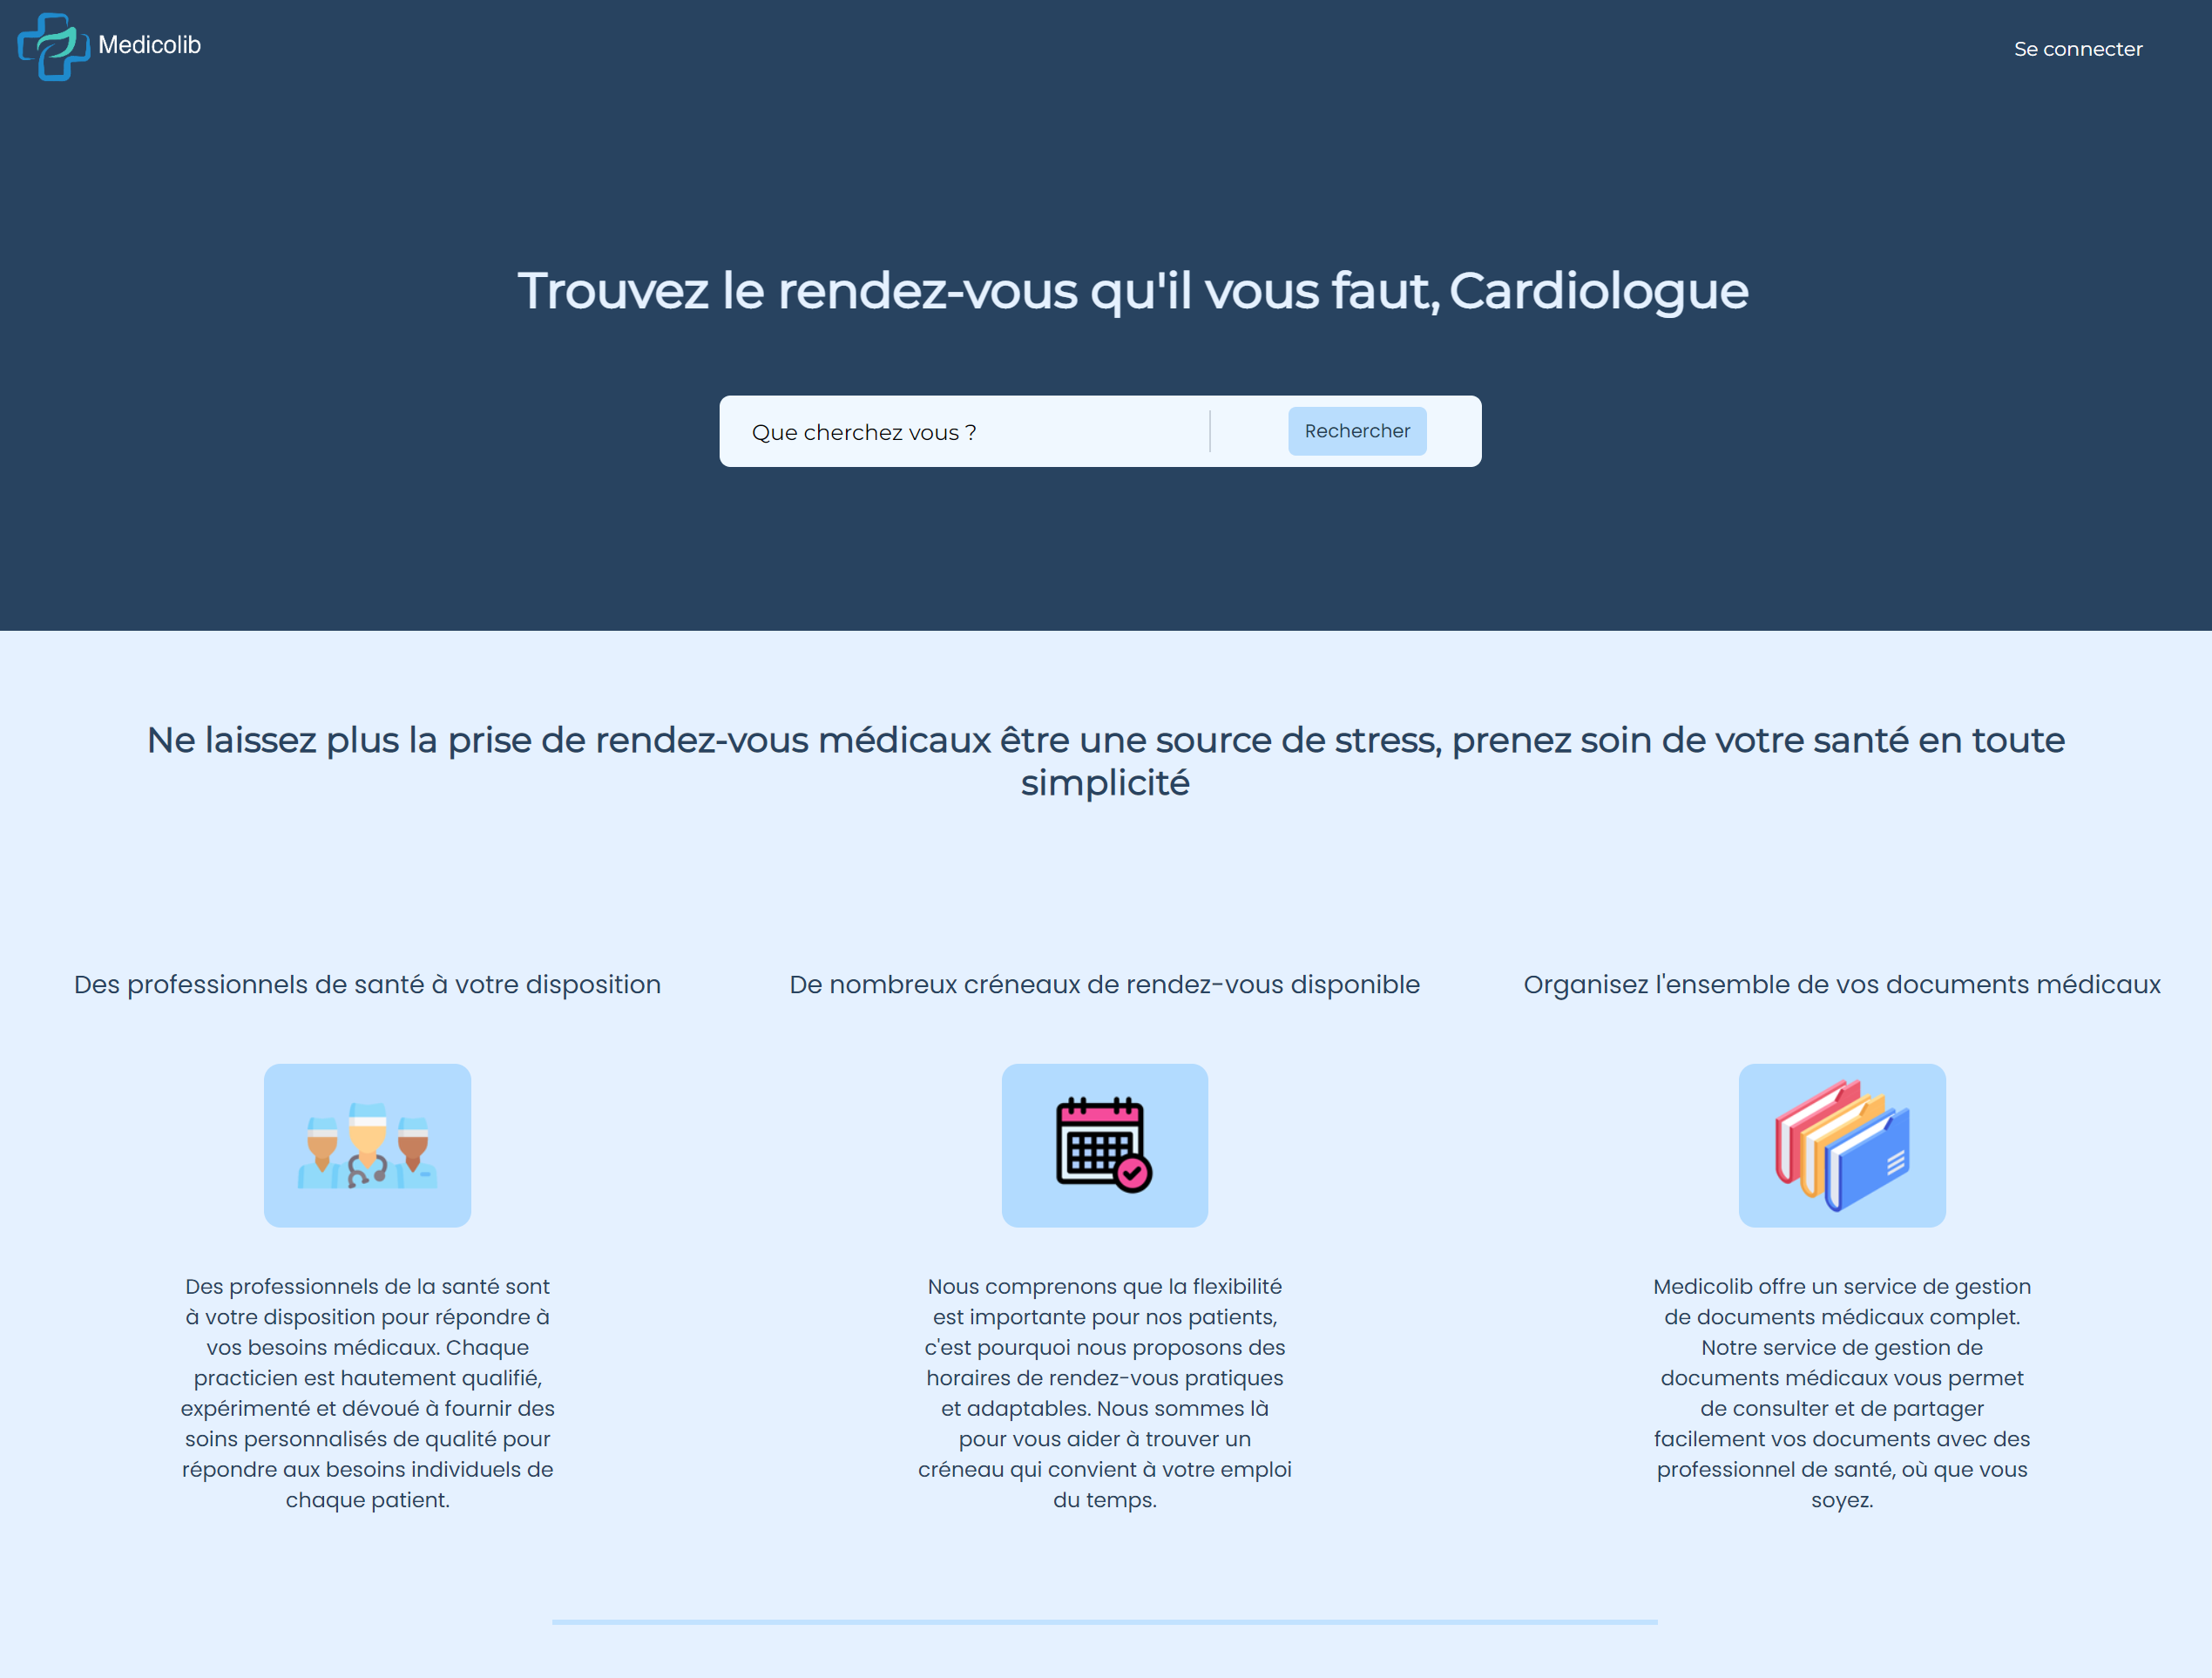
\includegraphics[width=0.8\textwidth]{captures/page-acceuil.png}
    \caption{\textit{\hyperref[homepage]{Page d'acceuil}}}
    \label{fig:DCU10}
\end{figure}

\subsection{Login}
\begin{figure}[H]
    \vspace{-10pt}
    \centering
    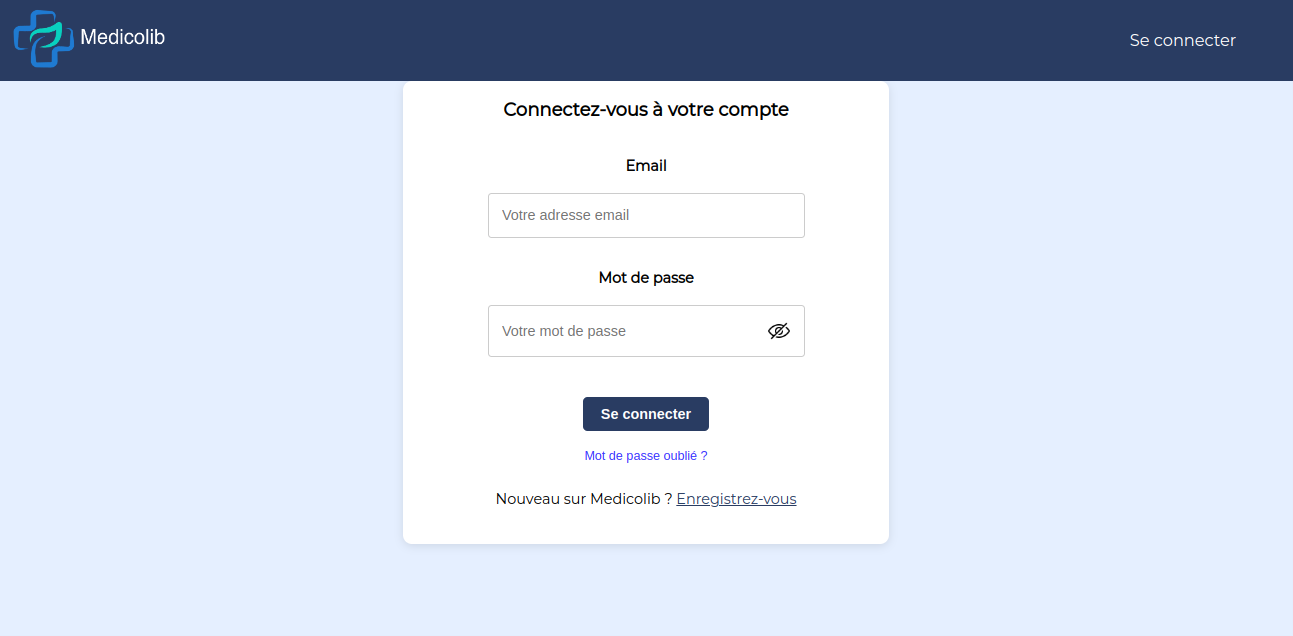
\includegraphics[width=0.8\textwidth]{captures/login.png}
    \caption{\textit{\hyperref[login]{Login}}}
    \label{fig:DCU11}
\end{figure}

\subsection{Register}
\begin{figure}[H]
    \vspace{-10pt}
    \centering
    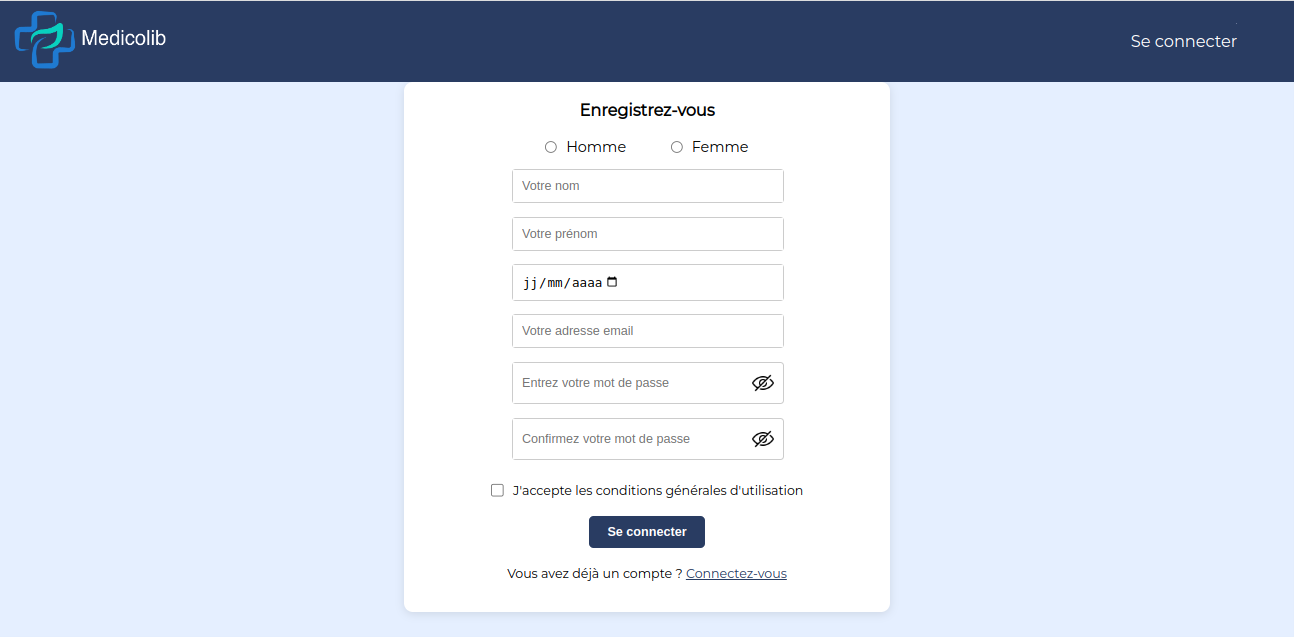
\includegraphics[width=0.8\textwidth]{captures/register.png}
    \caption{\textit{\hyperref[register]{Register}}}
    \label{fig:DCU12}
\end{figure}

\subsection{Patient Header}
\begin{figure}[H]
    \vspace{-10pt}
    \centering
    
\includegraphics[width=0.8\textwidth]{captures/patient-header.png}
    \caption{\textit{\hyperref[header]{Patient Header}}}
    \label{fig:DCU13}
\end{figure}

\subsection{Page des docteurs}
\begin{figure}[H]
    \vspace{-10pt}
    \centering
    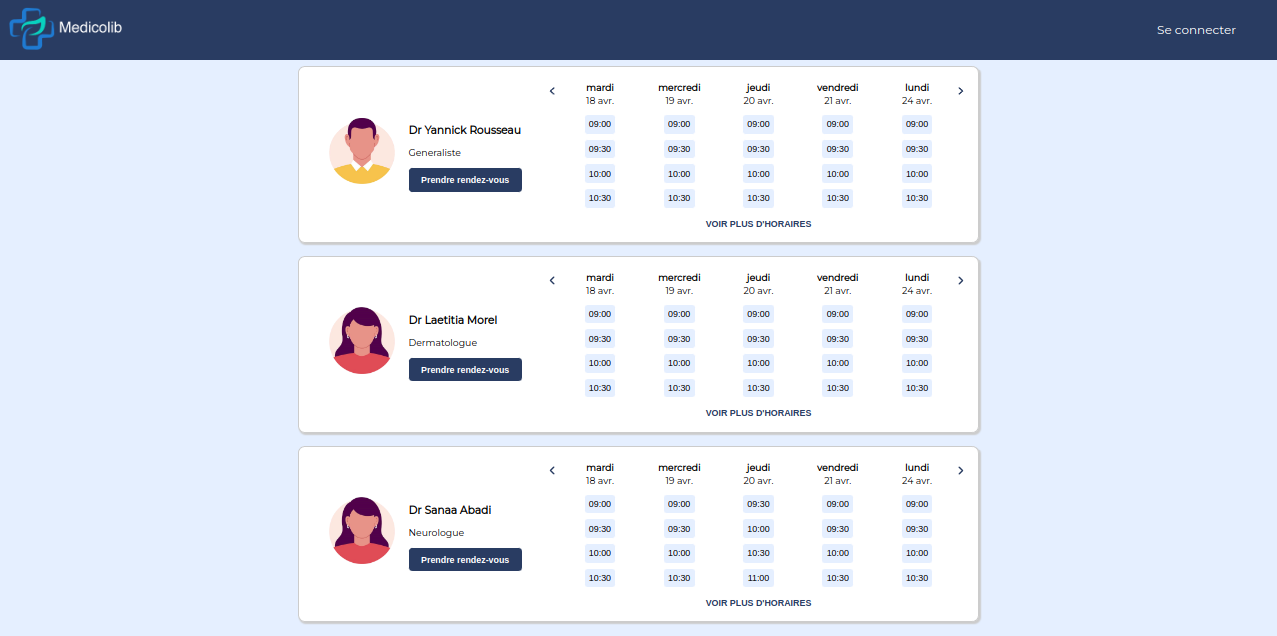
\includegraphics[width=0.8\textwidth]{captures/docteurs.png}
    \caption{\textit{\hyperref[docteurs]{Page des docteurs}}}
    \label{fig:DCU14}
\end{figure}

\subsection{Page de réservation d'un docteur}
\begin{figure}[H]
    \vspace{-10pt}
    \centering
    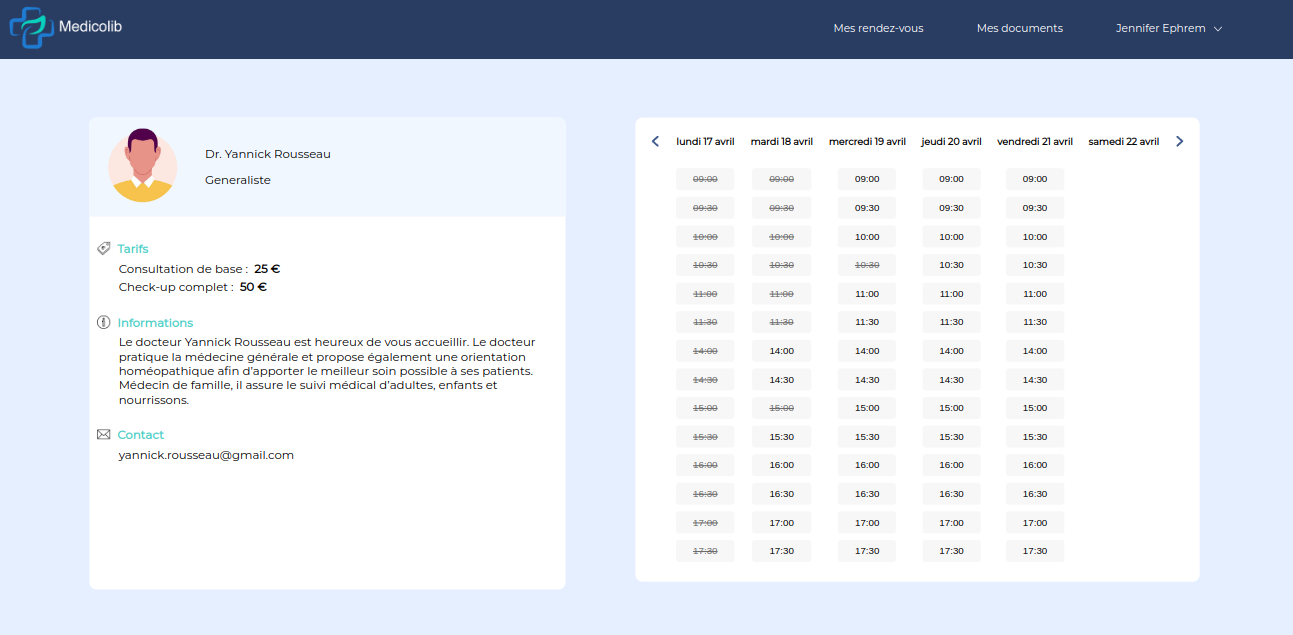
\includegraphics[width=0.8\textwidth]{captures/page-reservation-doctor.png}
    \caption{\textit{\hyperref[docteur]{Page de réservation d'un docteur}}}
    \label{fig:DCU15}
\end{figure}

\subsection{Page Mon Compte du patient}
\begin{figure}[H]
    \vspace{-10pt}
    \centering
    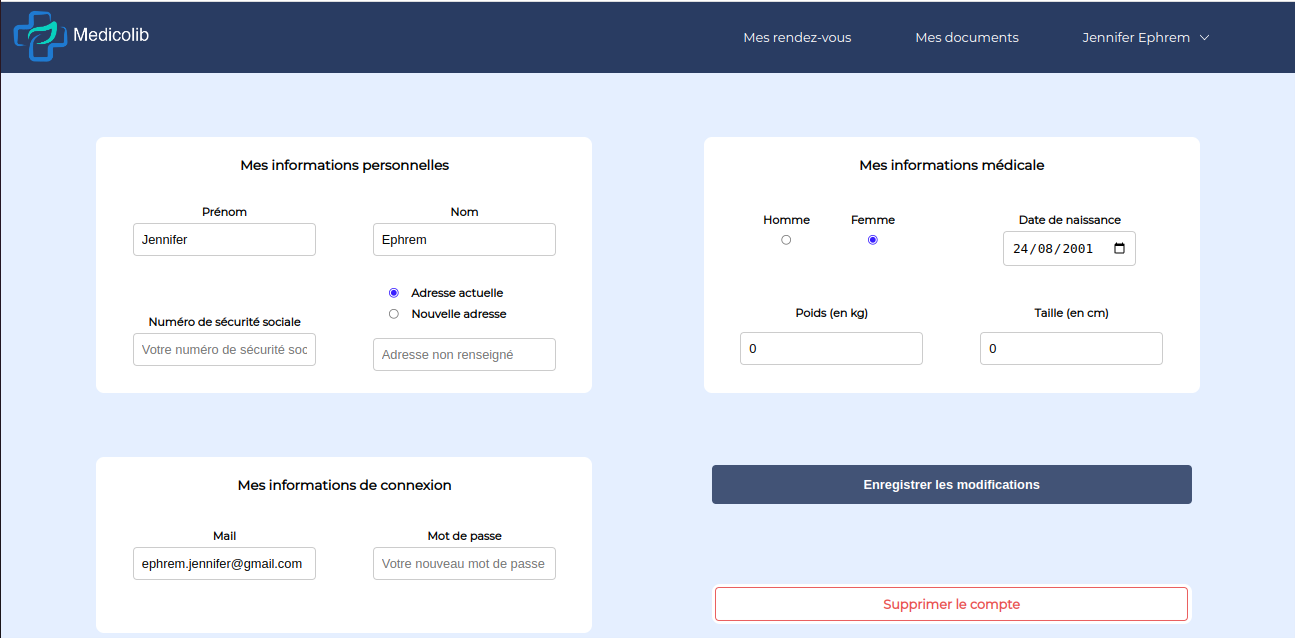
\includegraphics[width=0.8\textwidth]{captures/patient-edit-account.png}
    \caption{\textit{\hyperref[edit]{Page Mon Compte du patient}}}
    \label{fig:DCU16}
\end{figure}

\subsection{Page RDV du patient (lorsqu'il n'y a pas de RDV)}
\begin{figure}[H]
    \vspace{-10pt}
    \centering
    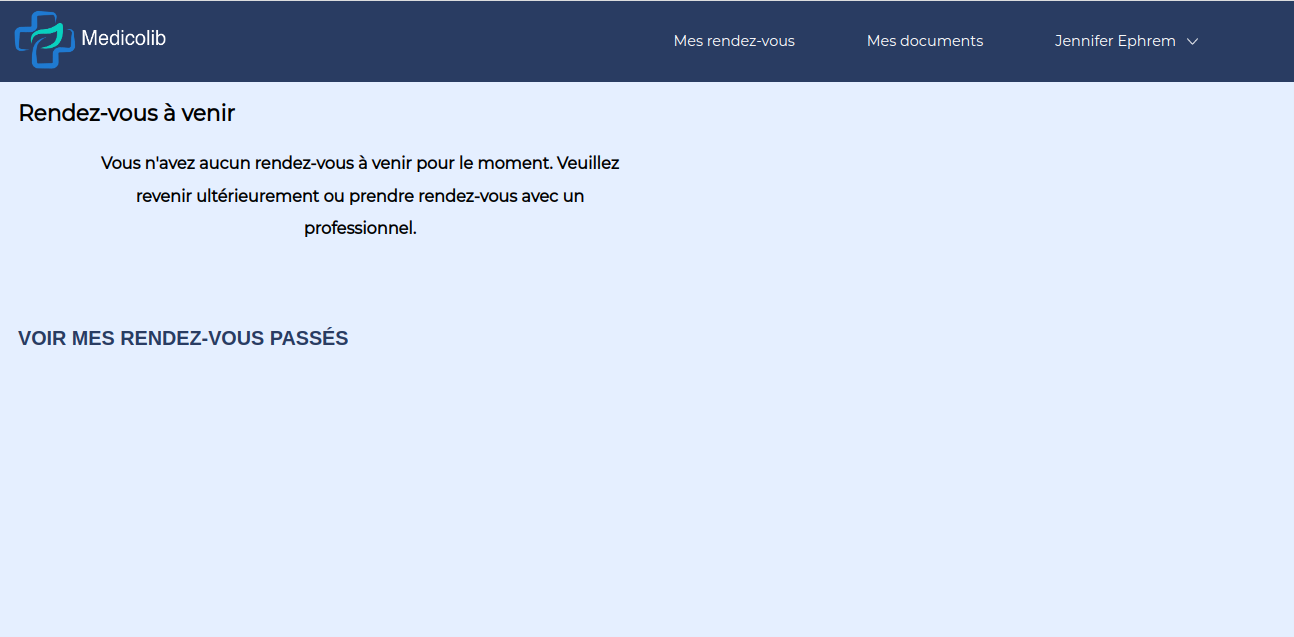
\includegraphics[width=0.8\textwidth]{captures/no-rdv.png}
    \caption{\textit{\hyperref[appointments]{Page RDV du patient}} (lorsqu'il n'y a pas de RDV)}
    \label{fig:DCU17}
\end{figure}

\subsection{Page RDV du patient}
\begin{figure}[H]
    \vspace{-10pt}
    \centering
    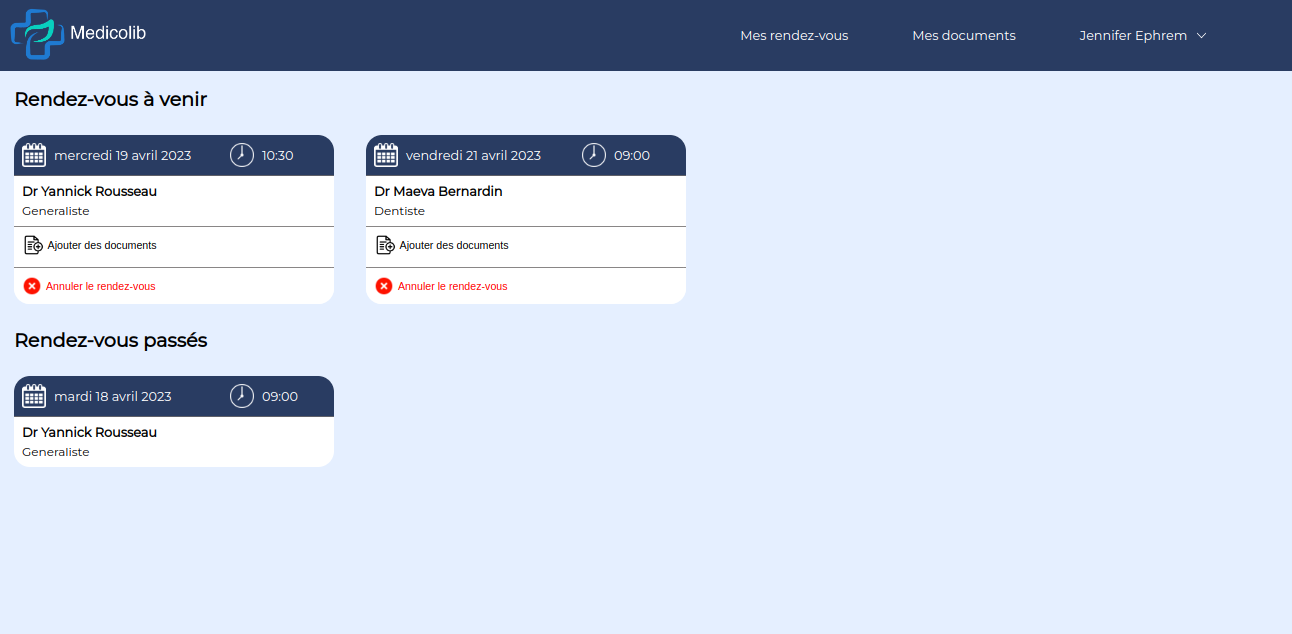
\includegraphics[width=0.8\textwidth]{captures/rdv-dispo.png}
    \caption{\textit{\hyperref[appointments]{Page RDV du patient}}}
    \label{fig:DCU18}
\end{figure}

\subsection{Confirmation de suppression d'un RDV}
\begin{figure}[H]
    \vspace{-10pt}
    \centering
    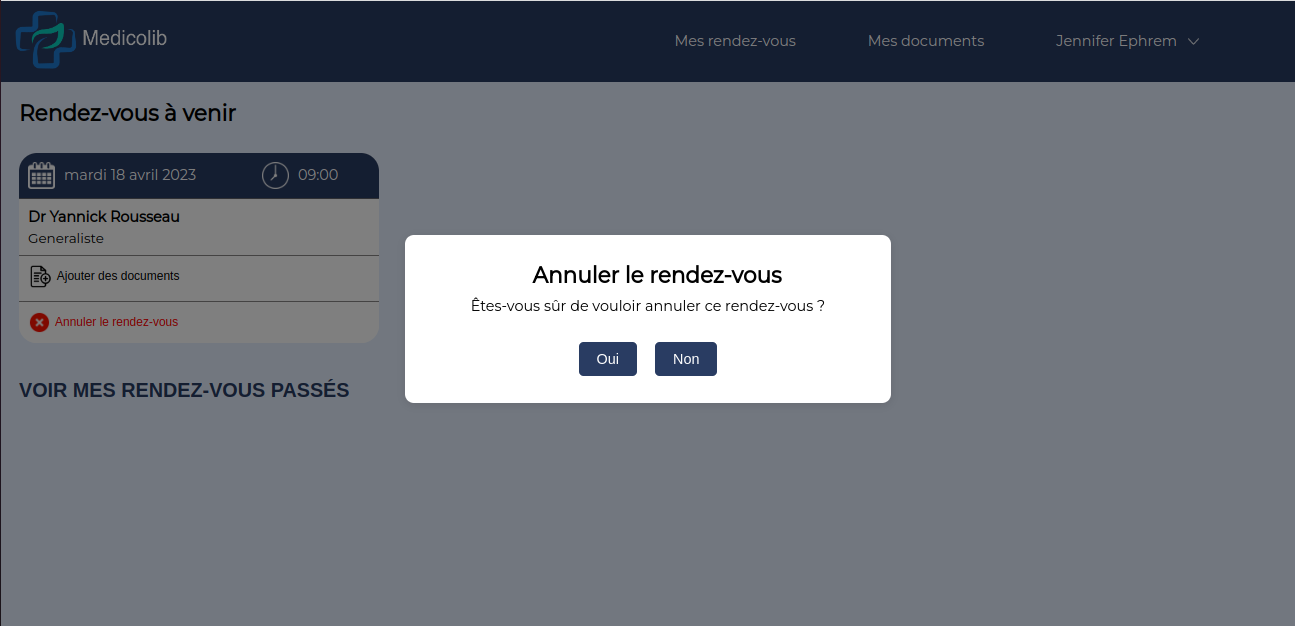
\includegraphics[width=0.8\textwidth]{captures/remove-rdv.png}
    \caption{Confirmation de suppression d'un RDV}
    \label{fig:DCU19}
\end{figure}

\subsection{Page Documents du patient (sans documents)}
\begin{figure}[H]
    \vspace{-10pt}
    \centering
    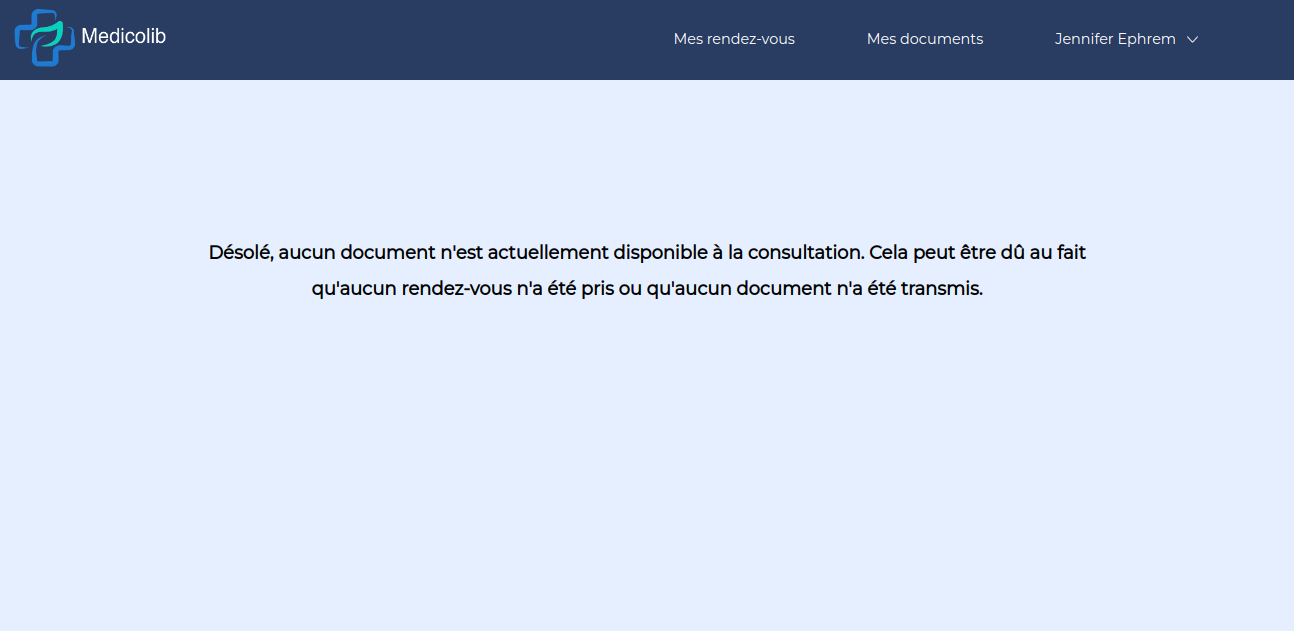
\includegraphics[width=0.8\textwidth]{captures/no-document.png}
    \caption{\textit{\hyperref[documents]{Page Documents du patient}} (sans documents)}
    \label{fig:DCU20}
\end{figure}

\subsection{Page Documents du patient}
\begin{figure}[H]
    \vspace{-10pt}
    \centering
    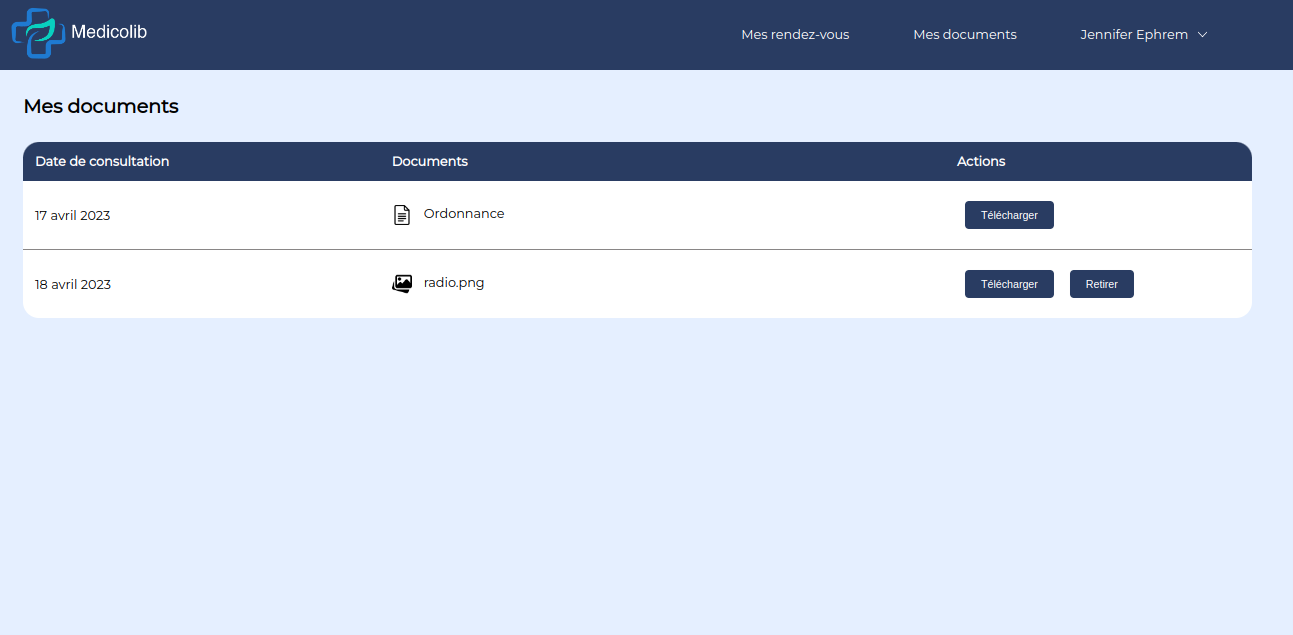
\includegraphics[width=0.8\textwidth]{captures/patient-document.png}
    \caption{\textit{\hyperref[documents]{Page Documents du patient}}}
    \label{fig:DCU21}
\end{figure}

\subsection{Doctor Header}
\begin{figure}[H]
    \vspace{-10pt}
    \centering
    
\includegraphics[width=0.8\textwidth]{captures/doctor-header.png}
    \caption{\textit{\hyperref[header2]{Doctor Header}}}
    \label{fig:DCU22}
\end{figure}

\subsection{Doctor Planning}
\begin{figure}[H]
    \vspace{-10pt}
    \centering
    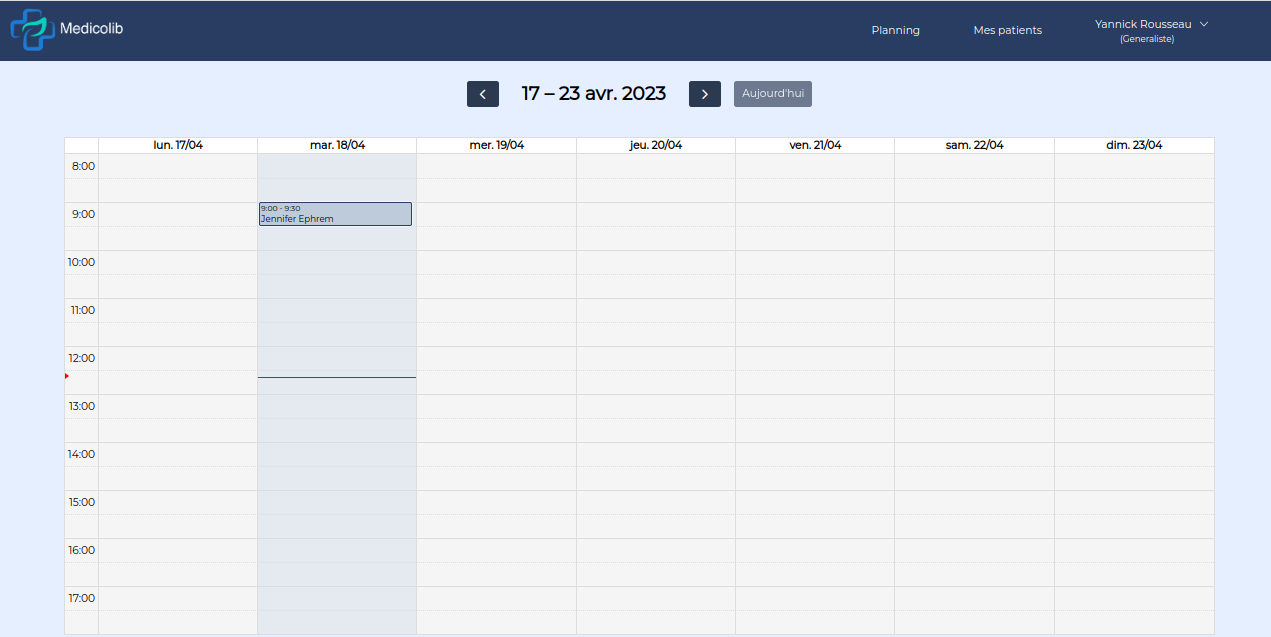
\includegraphics[width=0.8\textwidth]{captures/doctor-planning.png}
    \caption{\textit{\hyperref[planning]{Doctor Planning}}}
    \label{fig:DCU24}
\end{figure}

\subsection{RDV sur le planning du docteur}
\begin{figure}[H]
    \vspace{-10pt}
    \centering
    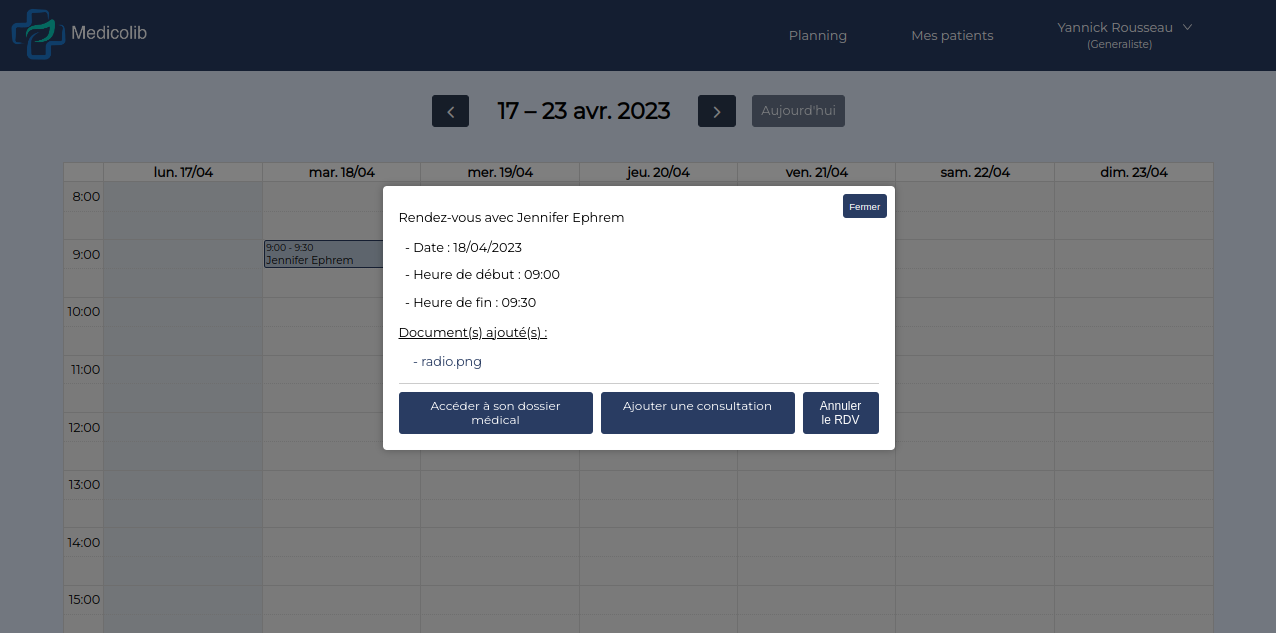
\includegraphics[width=0.8\textwidth]{captures/doctor-click-rdv.png}
    \caption{RDV sur le planning du docteur}
    \label{fig:DCU25}
\end{figure}

\subsection{Ajout d'une consultation sans prescription médicale}
\begin{figure}[H]
    \vspace{-10pt}
    \centering
    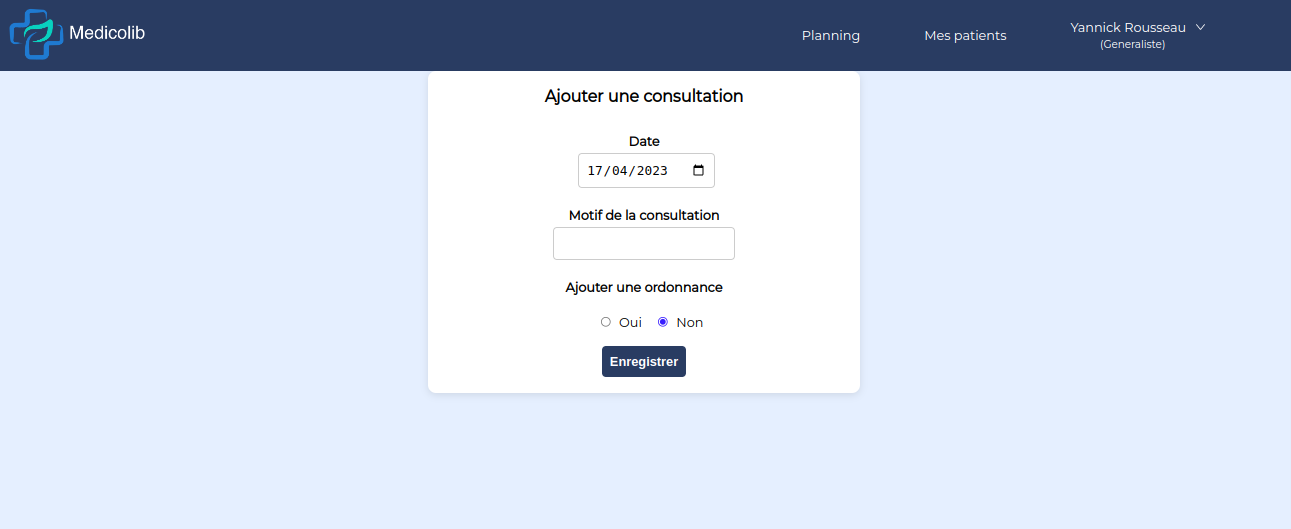
\includegraphics[width=0.8\textwidth]{captures/consultation-no-prescription.png}
    \caption{\textit{\hyperref[consultation]{Ajout d'une consultation}} sans prescription médicale}
    \label{fig:DCU26}
\end{figure}

\subsection{Ajout d'une consultation avec prescription médicale}
\begin{figure}[H]
    \vspace{-10pt}
    \centering
    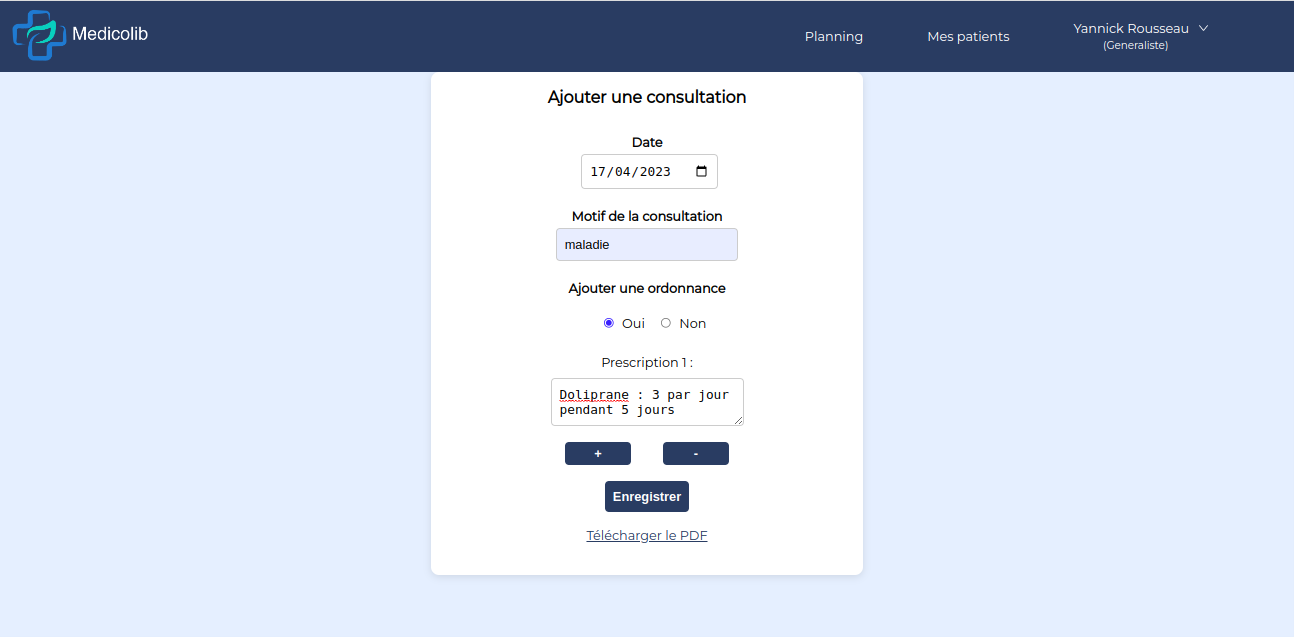
\includegraphics[width=0.8\textwidth]{captures/consultation-prescription.png}
    \caption{\textit{\hyperref[consultation]{Ajout d'une consultation}} avec prescription médicale}
    \label{fig:DCU27}
\end{figure}

\subsection{Prescription médicale}
\begin{figure}[H]
    \vspace{-10pt}
    \centering
    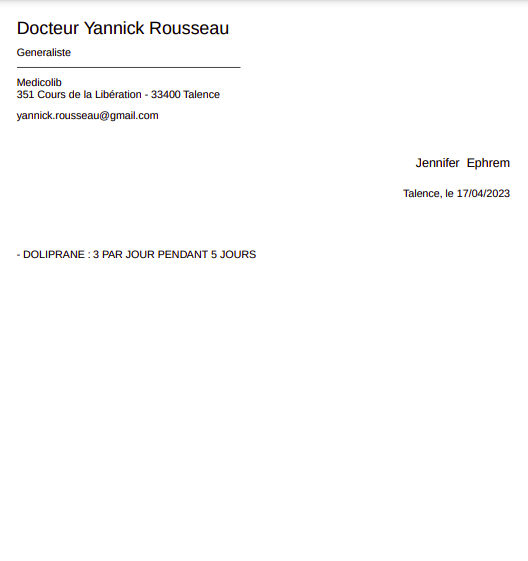
\includegraphics[width=0.7\textwidth]{captures/prescription.png}
    \caption{Prescription médicale}
    \label{fig:DCU28}
\end{figure}

\subsection{Page Mon Compte du docteur}
\begin{figure}[H]
    \vspace{-10pt}
    \centering
    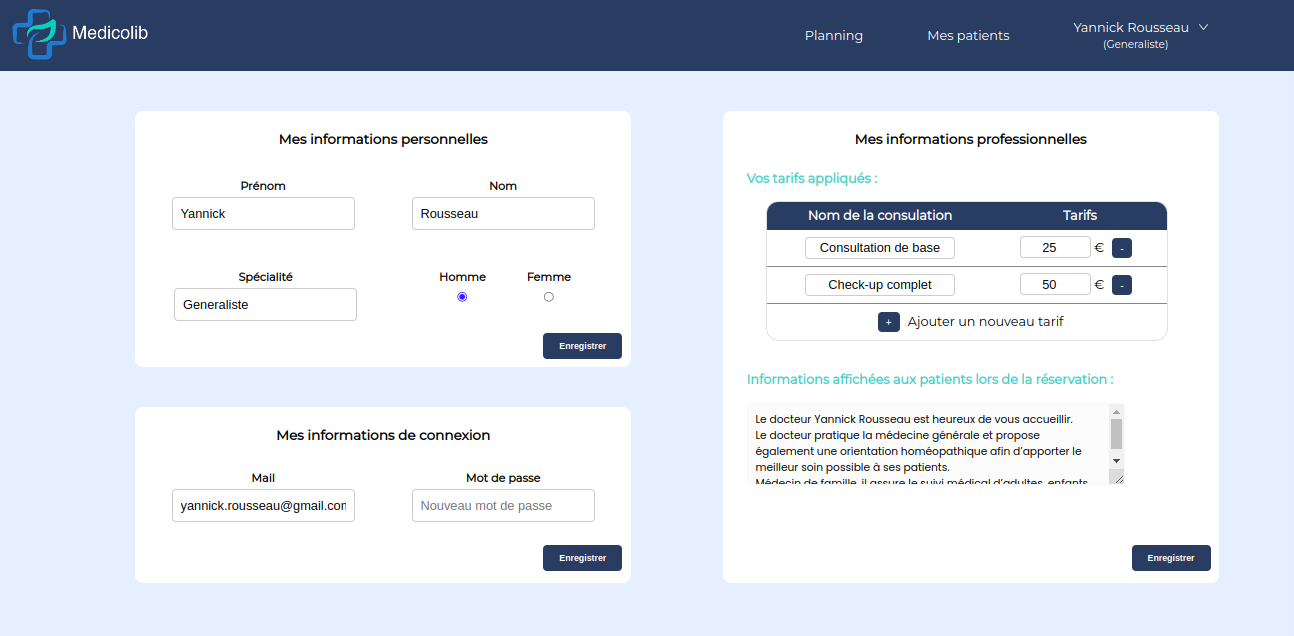
\includegraphics[width=0.8\textwidth]{captures/doctor-account.png}
    \caption{\textit{\hyperref[edit2]{Page Mon Compte du docteur}}}
    \label{fig:DCU29}
\end{figure}

\subsection{Envoie d'un mail}
\begin{figure}[H]
    \vspace{-10pt}
    \centering
    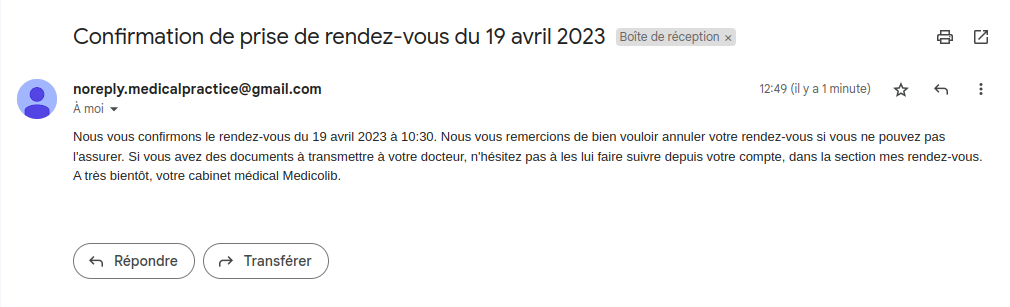
\includegraphics[width=0.8\textwidth]{captures/mail.png}
    \caption{Envoie d'un mail}
    \label{fig:DCU30}
\end{figure}

\chapter{Conclusion}

En conclusion, nous avons développé une application web pour un cabinet médical complète qui répond aux besoins spécifiques de ce secteur d'activité. Cette application permet aux 
médecins et aux patients de gagner du temps et de simplifier les processus de gestion des rendez-vous et des consultations 
médicales. \newline\newline
Au fil de notre projet, nous avons instauré une solution de gestion de rendez-vous à la fois facile et rapide pour nos patients. 
Ils peuvent désormais aisément planifier, annuler ou encore joindre des documents à leur rendez-vous. Les médecins, quant à eux, 
peuvent accéder aux dossiers médicaux et documents de leurs patients afin de leur prodiguer les soins les plus adaptés à leur situation. 
Ils bénéficient également d'une interface intuitive et conviviale pour visualiser leur emploi du temps, ainsi que la possibilité d'annuler un 
rendez-vous en cas d'indisponibilité. En un simple clic, l'ajout d'une consultation se fait aisément, avec la possibilité de télécharger une ordonnance 
en cas de prescription. Enfin, pour une gestion personnalisée, tous nos utilisateurs ont la possibilité de modifier leurs informations personnelles depuis 
l'onglet "Mon compte".\newline\newline
Cependant, bien que notre application soit une réussite, nous sommes conscients qu'il y a toujours place à l'amélioration. 
Parmi les perspectives d'amélioration, nous souhaitons renforcer la sécurité de nos utilisateurs en cryptant l'ensemble des données 
sensibles, notamment les dossiers médicaux, et non pas simplement les mots de passe. Nous voulons ainsi assurer la protection maximale 
des informations médicales de nos patients. 
Nous souhaitons également mettre en place un sytème de téléconsultation pour que les patients puissent bénéficier 
des soins nécessaires directement depuis chez eux. Enfin, dans le contexte de notre application web,  notre objectif serait de réduire au maximum 
les risques d'injections SQL dans notre base de données afin d'assurer la fiabilité et la confidentialité des données. \newline\newline
Dans l'ensemble, nous sommes fiers de ce que nous avons accompli avec cette application web pour un cabinet médical. Nous sommes 
convaincus que notre solution répondra aux besoins des médecins et des patients, et nous sommes impatients de recevoir les commentaires 
et les suggestions de nos utilisateurs pour continuer à améliorer notre application.


\bibliography{biblio}

\end{document}